\documentclass{article}
\usepackage{amsmath} %This allows me to use the align functionality.
                     %If you find yourself trying to replicate
                     %something you found online, ensure you're
                     %loading the necessary packages!
\usepackage{amsfonts}
\usepackage{lineno}
\linenumbers
\usepackage[margin=1.0in]{geometry}
\usepackage{float}
\usepackage{slashbox}
\usepackage{graphicx}
\usepackage{multicol}
\newcommand{\nCr}[2]{\,_{#1}C_{#2}} % nCr
\newcommand{\nPr}[2]{\,_{#1}P_{#2}} % nPr
\usepackage{natbib}        %For the bibliography
\bibliographystyle{apalike}%For the bibliography
\usepackage{Sweave}
\begin{document}
\Sconcordance{concordance:part2.tex:part2.Rnw:%
1 17 1 1 0 5 1 1 3 5 0 1 2 27 1 1 2 5 0 1 3 6 1 1 9 11 0 1 2 1 9 11 0 1 %
2 6 1 1 3 2 0 1 2 1 0 1 2 1 0 2 1 3 0 1 2 14 1 1 3 2 0 1 9 8 0 1 9 8 0 %
1 1 1 2 4 0 1 2 20 1 1 2 1 0 1 1 1 12 11 0 1 12 11 0 1 1 3 0 1 2 10 1 1 %
-12 1 17 5 1 1 2 1 0 4 1 3 0 1 2 14 1 1 5 4 0 1 1 1 3 2 0 2 1 15 0 1 2 %
8 1 1 2 1 0 2 1 1 3 2 0 1 3 2 0 1 13 15 0 1 2 2 1 1 -4 1 9 12 1 1 3 5 0 %
1 2 14 1 1 3 2 0 2 1 1 12 14 0 1 2 2 1 1 -4 1 9 18 1 1 5 4 0 1 4 3 0 1 %
4 3 0 3 1 8 0 1 2 16 1 1 2 1 0 1 7 6 0 2 1 1 2 3 0 1 2 16 1 1 2 10 0 1 %
2 6 1 1 2 1 0 1 1 1 2 16 0 1 2 24 1 1 6 5 0 1 1 15 0 1 2 14 1 1 6 5 0 1 %
1 15 0 1 2 14 1 1 6 5 0 1 1 15 0 1 2 14 1 1 6 5 0 1 1 15 0 1 2 14 1 1 2 %
4 0 1 2 10 1 1 3 2 0 2 1 1 11 13 0 1 2 2 1 1 -4 1 9 15 1 1 2 1 0 3 1 1 %
5 3 0 3 1 8 0 1 2 15 1 1 2 1 0 1 7 6 0 2 1 3 0 1 2 16 1 1 2 10 0 1 2 14 %
1 1 2 4 0 1 2 16 1 1 3 2 0 1 3 2 0 1 1 1 11 13 0 1 2 2 1 1 -4 1 9 27 1 %
1 4 3 0 1 3 2 0 1 4 3 0 3 1 8 0 1 2 16 1 1 2 1 0 1 7 6 0 2 1 3 0 1 2 20 %
1 1 2 10 0 1 2 4 1 1 2 1 0 1 1 1 2 16 0 1 2 22 1 1 6 5 0 1 1 15 0 1 2 %
14 1 1 6 5 0 1 1 15 0 1 2 28 1 1 3 2 0 1 2 4 0 1 2 46 1 1 3 2 0 1 3 2 0 %
2 1 1 16 15 0 1 3 1 0 2 1 1 18 17 0 1 2 3 0 1 2 28 1 1 9 8 0 1 9 7 0 1 %
9 7 0 1 5 3 0 3 1 9 0 1 2 15 1 1 2 1 0 1 7 6 0 3 1 9 0 1 2 30 1 1 2 10 %
0 1 2 4 1 1 2 1 0 1 1 1 2 16 0 1 2 10 1 1 8 21 0 1 2 4 1 1 8 21 0 1 2 4 %
1 1 8 21 0 1 2 4 1 1 8 21 0 1 2 14 1 1 9 8 0 1 9 7 0 1 9 7 0 1 5 3 0 3 %
1 9 0 1 2 15 1 1 2 1 0 1 7 6 0 2 1 3 0 1 2 30 1 1 2 10 0 1 2 14 1 1 3 2 %
0 1 2 4 0 1 2 35 1 1 3 2 0 1 2 1 0 2 1 1 14 13 0 1 4 2 0 2 1 1 14 13 0 %
1 2 3 0 1 2 24 1 1 9 8 0 1 9 7 0 1 5 3 0 3 1 8 0 1 2 15 1 1 2 1 0 1 7 6 %
0 2 1 3 0 1 2 25 1 1 2 10 0 1 2 10 1 1 9 8 0 1 9 7 0 1 5 3 0 3 1 8 0 1 %
2 15 1 1 2 1 0 1 7 6 0 3 1 8 0 1 2 25 1 1 2 10 0 1 2 10 1 1 3 2 0 1 2 4 %
0 1 2 33 1 1 3 2 0 1 2 1 0 1 3 2 0 1 1 1 13 12 0 1 3 1 0 1 2 1 0 1 1 1 %
13 12 0 1 2 3 0 1 2 24 1 1 7 6 0 1 7 5 0 1 5 3 0 3 1 8 0 1 2 15 1 1 2 1 %
0 1 7 6 0 2 1 3 0 1 2 26 1 1 2 10 0 1 2 2 1 1 2 1 0 1 1 1 2 16 0 1 2 10 %
1 1 6 18 0 1 2 4 1 1 6 18 0 1 2 4 1 1 6 18 0 1 2 10 1 1 7 6 0 1 7 5 0 1 %
5 3 0 3 1 8 0 1 2 15 1 1 2 1 0 1 7 6 0 2 1 3 0 1 2 27 1 1 2 10 0 1 2 10 %
1 1 3 2 0 1 2 4 0 1 2 51 1 1 2 1 0 2 1 1 13 12 0 1 13 12 0 1 1 3 0 1 2 %
2 1 1 -4 1 9 36 1 1 3 11 0 1 2 6 1 1 3 11 0 1 2 4 1 1 2 1 0 1 2 1 0 1 3 %
12 0 1 2 12 1 1 3 2 0 1 2 4 0 1 2 31 1 1 2 1 0 2 1 1 13 12 0 1 13 12 0 %
1 1 3 0 1 2 2 1 1 -4 1 9 32 1 1 3 11 0 1 2 6 1 1 3 11 0 1 2 8 1 1 3 2 0 %
1 2 4 0 1 2 41 1 1 2 1 0 2 1 1 13 12 0 1 13 12 0 1 1 3 0 1 2 2 1 1 -4 1 %
9 36 1 1 3 11 0 1 2 4 1 1 2 1 0 1 2 1 0 1 3 11 0 1 2 10 1 1 3 11 0 1 2 %
43 1 1 2 1 0 1 1 3 0 1 2 6 1}

%set the size of the graphs to fit nicely on a 8.5x11 sheet
\noindent \textbf{MA 354: Data Analysis I -- Fall 2019}\\%\\ gives you a new line
\noindent \textbf{Exam 2:}\vspace{1em}\\

\begin{Schunk}
\begin{Sinput}
> dat.HOA<-read.table("https://cipolli.com/students/data/Exam1Data.txt",
+               header=T,sep=",")
\end{Sinput}
\end{Schunk}

\textbf{Name:} Sahil Lalwani\\

Suburban areas play an integral role in the development of sustainable cities; however, developers often do not consider sustainability in the construction of subdivisions and the subsequent adoption of homeowner's association (HOA) covenants. While there are multiple actions homeowners can take to contribute to personal sustainability on the plot-by-plot level, these actions are not always adopted or supported by greater neighborhood norms. \\

The current literature provides assessments of individual sustainability indicators at the homeowner and neighborhood level as well as multi-indicator sustainability assessments of cities and larger metropolitan areas but lacks such multi-indicator analyses at the homeowner and neighborhood level. This study assesses the relationship among multiple sustainability indicators of homeowner behavior including recycling habits, lawn care, tree planting, and home gardening, and compares these behaviors between neighborhoods with HOAs and those without. Data metrics were collected from twelve neighborhoods in Greenville, South Carolina through on-site observation, analysis of Google Earth images, and qualitative assessment of HOA covenants.\\

The data for this report consists of 1,616 observations of homes in Greenville, SC and the seven variables recorded for each. 
Basic descriptions of the variables and other important information can be found below.
\begin{itemize}
\item \textbf{Neighborhood:} This reports which of the 12 neighborhoods in Greenville, SC each observed home is located. There are no missing values for this variable. 
\item \textbf{Lot Number:} This reports the lot number of the homes. There are no missing values for this variable. 
\item \textbf{HOA:} This reports whether or not the homes are part of a homeowners' association (1 = yes; 2 = no). There are no missing values for this variable.
\item \textbf{Recycle:} This reports the recycling status of the homes (1 = both recycling bin and trash bin present at the home; 2 = only a trash bin was present). There are 274 missing values for this variable. These missing values correspond to neighborhoods with no curb side pick up (i.e., Brownstone, Edgewood, Glastonbury, and Fox Springs).
\item \textbf{Lawn Care:} This represents a likert variable on a scale of 1 to 4 (1 = excellent; 2 = good; 3= poor; 4 = none). This measure
maps onto how artificially managed the lawn is where 1 means the lawns were highly artificially managed with presumed regular chemical application and 4 means the lawns were naturally managed (i.e., not managed at all). There are no missing values for this variable.
\item \textbf{Trees:} This represents the number of trees in the front yard. There are 14 missing values for this variable. 
\item \textbf{Garden:} This represents whether a garden was present in the front or back of the homes (1 = yes; 2 = no). There are no missing values for this variable.
\end{itemize}

%%%%%%%%%% Write your solution here %%%%%%%%%%

All of the analysis in this report has been done using the R language (\cite{rstandard}) and the relevant packages associated with it. 

\section*{Data Cleaning}

Since tree planting is a specific element within our multiple sustainability indicators, we can remove 14 observations which have missing values for the variable Trees to obtain a dataset which will be used for any analysis throughout that includes the variable \textbf{Trees}.

\begin{Schunk}
\begin{Sinput}
> dat.HOAn<-subset(dat.HOA, !is.na(dat.HOA$Trees)) # Remove observations where Trees variable 
>                                                  # has missing values
\end{Sinput}
\end{Schunk}

The missing values for the variable \textbf{Recycle} result from the fact that the recycling status of homes in neighborhoods with no curb side pick up (that is, Brownstone, Edgewood, Glastonbury and Fox Springs) is unobservable with the method employed by the researcher to collect data and record values of variable Recycle for the study.\\

In fact, it is quite possible that households with missing values for the variable \textbf{Recycle} likely have some trash storage and even some arrangement for recycling by taking personal initiative to drive. It must be noted that while the method of data collection fails to address recycling status of 274 households, the possibility of varied recycling tendencies and initiatives among these households demonstrate that none of the levels of the variable \textbf{Recycle} that is, 1 or 2, is appropriate or broad enough to be associated with these 274 observations. \\

Thus, it seems appropriate to categorize the recycling status of these 274 households as level 3 (\textbf{Recycle}=3) for a major reason. The houses with no curb side pick up account for roughly 17\% of all observations in the given data and including them as part of the broader analysis brings selectivity and focus to our approach.

\begin{Schunk}
\begin{Sinput}
> for (i in 1:1602){
+   if(is.na(dat.HOAn$Recycle[i])==TRUE){
+     dat.HOAn$Recycle[i]=3 # Recycle category=3 for NA values for dat.HOAn
+   }
+   else{
+     dat.HOAn$Recycle[i]=dat.HOAn$Recycle[i]
+   }
+ }
\end{Sinput}
\end{Schunk}

\begin{Schunk}
\begin{Sinput}
> for (i in 1:1602){
+   if(is.na(dat.HOA$Recycle[i])==TRUE){
+     dat.HOA$Recycle[i]=3 # Recycle category=3 for NA values for dat.HOA
+   }
+   else{
+     dat.HOA$Recycle[i]=dat.HOA$Recycle[i]
+   }
+ }
\end{Sinput}
\end{Schunk}

\section*{Data Analysis}

\section*{Trees}

The study defines tree planting as a sustainability indicator of homeowner behavior. In this section, we use graphical summaries and numerical evidence to understand how tree planting tendencies differ between neighborhoods with HOAs and those without. The following is a brief description of our sample data:

\begin{Schunk}
\begin{Sinput}
> # Table for sample data for dat.HOAn
> trees_sample<-data.frame()
> one<-list(1,"Yes", nrow(subset(dat.HOAn,dat.HOAn$HOA==1)),nrow(subset(dat.HOA,
+           is.na(dat.HOA$Trees)==TRUE & dat.HOA$HOA==1)))
> two<-list(2,"No", nrow(subset(dat.HOAn,dat.HOAn$HOA==2)),nrow(subset(dat.HOA,
+           is.na(dat.HOA$Trees)==TRUE & dat.HOA$HOA==2)))
> trees_sample<-rbind(trees_sample,one,two)
> colnames(trees_sample)<-c("Value","Status","Num_homes","Rm_homes") # Column names for table
\end{Sinput}
\end{Schunk}


\begin{table}[H]
  \centering
    \begin{tabular}{lcccc|}\hline
    HOA Value & HOA status & Number of houses & $\begin{matrix} \text{Number of houses with}\\ \text{missing values removed} \end{matrix}$ \\\hline
    1&Yes& 1056& 3\\
     2&No& 546& 11\\\hline
  \textbf{Total}&&1602&14\\\hline
    \end{tabular}
    \caption{Description of sample data for comparing tree planting tendency between HOA and non-HOA households}
  \end{table}

Considering \textbf{Tree} is the only quantitative variable among 6 other categorical variables in the data provided, we compare detailed numerical summaries for the variable \textbf{Trees} for neighborhoods with HOA and those without to understand the respective distributions of the data on the variable \textbf{Trees} for each HOA status and the center, spread, shape and deviations from the overall pattern for each distribution. 

\begin{Schunk}
\begin{Sinput}
> # Dataframe for summary of data that include mean, sd, median, IQR, quantiles and max
> trees_summary<-data.frame()
> one<-list(1,"Yes", round(mean(subset(dat.HOAn, dat.HOAn$HOA==1)$Trees),3),
+           round(sd(subset(dat.HOAn, dat.HOAn$HOA==1)$Trees),3),
+           round(median(subset(dat.HOAn, dat.HOAn$HOA==1)$Trees),3),
+           round(IQR(subset(dat.HOAn, dat.HOAn$HOA==1)$Trees),3),
+           round(quantile(subset(dat.HOAn, dat.HOAn$HOA==1)$Trees,0.25),3),
+           round(quantile(subset(dat.HOAn, dat.HOAn$HOA==1)$Trees,0.75),3),
+           round(max(subset(dat.HOAn, dat.HOAn$HOA==1)$Trees),3),
+           length(boxplot(subset(dat.HOAn, dat.HOAn$HOA==1)$Trees)$out),
+           min(boxplot(subset(dat.HOAn, dat.HOAn$HOA==1)$Trees)$out))
> two<-list(2,"No", round(mean(subset(dat.HOAn, dat.HOAn$HOA==2)$Trees),3),
+           round(sd(subset(dat.HOAn, dat.HOAn$HOA==2)$Trees),3),
+           round(median(subset(dat.HOAn, dat.HOAn$HOA==2)$Trees),3),
+           round(IQR(subset(dat.HOAn, dat.HOAn$HOA==2)$Trees),3),
+           round(quantile(subset(dat.HOAn, dat.HOAn$HOA==2)$Trees,0.25),3),
+           round(quantile(subset(dat.HOAn, dat.HOAn$HOA==2)$Trees,0.75),3),
+           round(max(subset(dat.HOAn, dat.HOAn$HOA==2)$Trees),3),
+           length(boxplot(subset(dat.HOAn, dat.HOAn$HOA==2)$Trees)$out),
+           min(boxplot(subset(dat.HOAn, dat.HOAn$HOA==2)$Trees)$out))
> trees_summary<-rbind(trees_summary,one,two)
> colnames(trees_summary)<-c("Value","Status","Mean","Sd","Median","IQR",
+                            "1Q","3Q","Max","num_out", "min_out")
\end{Sinput}
\end{Schunk}

\begin{table}[H]
  \centering
    \begin{tabular}{lccccccc|}\hline
    HOA Value & HOA status & Mean SD & Median IQR & 1st Qu. & 3rd Qu. & Max \\\hline\hline
    1 & Yes & $2.947 \pm 2.668$
    & $2 \pm
    3$&1&4&
    35\\
    
    2 & No & $5.896 \pm 5.172$
    & $5 \pm
    6$&2&8&
    40\\
    
    \end{tabular}
    \caption{Numerical summary for \textbf{Trees} by HOA status}
  \end{table}

We use the ggplot2 package ({\cite{ggplot2q}}) and GridExtra package ({\cite{gride}}) to construct relevant graphs for visualization of data.

\begin{Schunk}
\begin{Sinput}
> library("ggplot2") 
> library("gridExtra")
> p1<-ggplot(dat.HOAn, aes(x=as.factor(HOA), y=Trees)) + 
+   geom_violin(fill="lightblue",    
+               trim = FALSE,
+               alpha = 0.9, 
+               show.legend = FALSE,
+               position=position_dodge(width=0.9))+
+   geom_boxplot(width = 0.15, fill="white", position=position_dodge(width=0.9))+
+   #plot smaller boxplot inside violin
+   xlab("HOA Status (1=Yes, 2=No)")+ #x axis label
+   ylab("Number of Trees")    + #y axis label
+   ggtitle("Number of Trees in the front yard", subtitle = "1056 households with HOA=1 and 564 households\nwith HOA=2") + #add title to plot
+   theme_bw()  #removes grey background 
> p2<-ggplot(data=dat.HOAn, 
+            aes(x=Trees,fill=as.factor(HOA)))+ #which data to plot
+   geom_density(alpha = 0.2)+
+   xlab("Number of Trees")+ #x axis label
+   ylab("Density")+ #y axis label
+   ggtitle("Number of Trees in the front yard",
+           subtitle = "1056 households with HOA=1 and 564 households\nwith HOA=2") + #add title to plot
+   theme_bw()+ #removes grey background 
+   geom_hline(yintercept=0)+  #adds a line for the x-axis
+   scale_fill_manual(values=c("red", "blue", "grey"))+
+   xlim(-2,40)+
+   labs(fill="HOA Status")
> grid.arrange(p1,p2,ncol=2)
\end{Sinput}
\end{Schunk}

\textbf{Numerical summary and visual evidence}: 

From the numerical summary in Table 2, it seems that the tree planting tendency is relatively higher and more varied across households that are not part of HOA compared to households that are part of HOA. The median number of trees planted by houses not members of HOA is 5, which is significantly higher than 2 trees as the median number of trees planted by houses which are HOA members. The average number of trees planted by non-HOA members is 6 (approx.) which is also higher than 3(approx.) as the average number of trees planted by HOA members.\\

Note that the relatively higher variation in planting tendency among non-HOA households is also evident through their higher values of IQR and SD (5.172 and 6 respectively) compared to those for HOA households (2.668 and 3 respectively).\\

We now visualize the data to understand the numerical summaries in context to the distribution of data for both groups of households with different HOA status. \\

\begin{figure}[H]
\centering
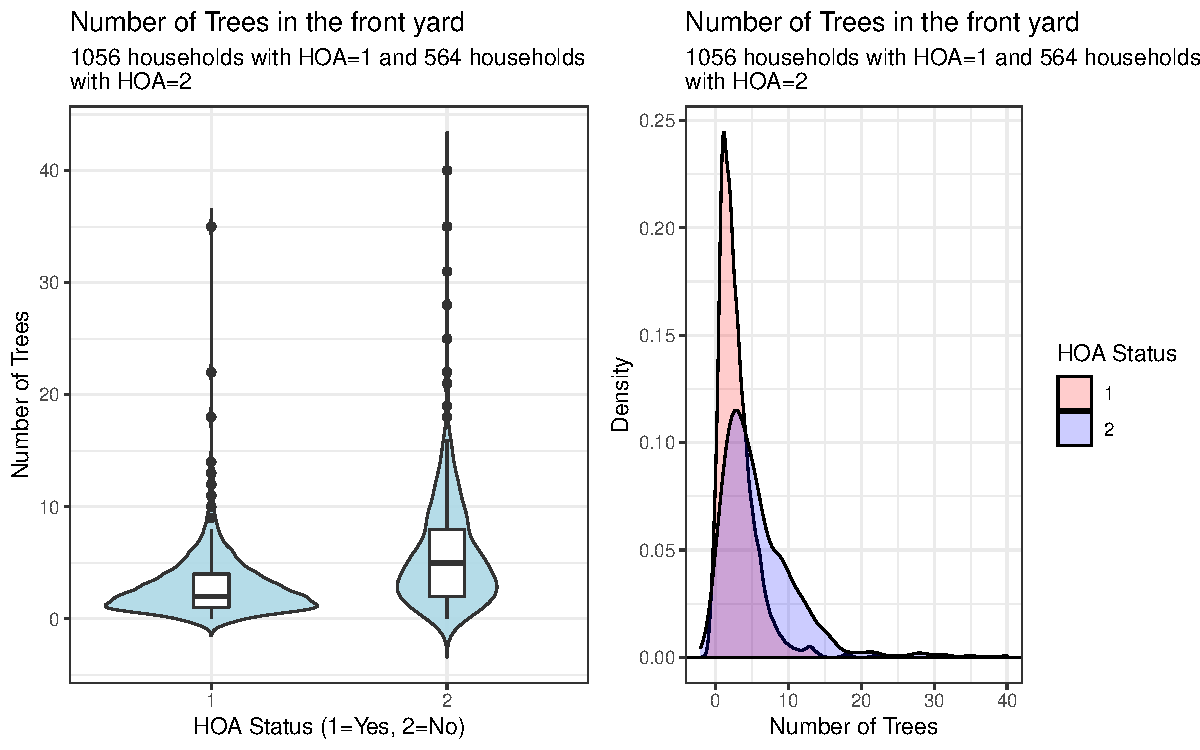
\includegraphics{part2-008}
\caption{Distribution of data from dat.HOAn for number of trees in the front yard for n=1602 households categorized by HOA status. \textbf{Left:} Violin plot \textbf{Right:} Density plot} \label{Fig:Plot1}
\end{figure}

The box plots help visualize the higher median and IQR for non-HOA households compared to HOA households. Note that the plot on the right illustrates that the density plots for number of trees for both HOA and non-HOA households are highly right skewed.\\

To compare the skewness of of the density plots,
\begin{Schunk}
\begin{Sinput}
> library("e1071")
> hoa<-skewness(subset(dat.HOAn, dat.HOAn$HOA==1)$Trees)
> hoa<-round(hoa,2)
> not_hoa<-skewness(subset(dat.HOAn, dat.HOAn$HOA==2)$Trees)
> not_hoa<-round(not_hoa,2)
\end{Sinput}
\end{Schunk}

The skewness for the density plot for number of trees for HOA households is 3.31 while it is 2.23 for the other. Thus, the plot is slightly more right skewed for households that are a part of HOA. The box plot also helps visualize numerical evidence for the fact that the average number of trees are greater for non-HOA households compared to HOA households.\\

The highly skewed nature of both plots implies that a very small proportion of HOA and non-HOA households plant a very large number of trees relative to other households within their respective HOA status category. This necessitates the need to use the median number of trees planted to compare tree planting tendencies between HOA and non-HOA households.\\

Even though there is higher variation in number of trees planted among non-HOA households, we use the analysis from visual and numerical summaries of data to claim that tree planting tendencies may be higher, in terms of median number of trees planted, among non-HOA households.\\

\textbf{Testing visual "evidence" for statistical validity}:

In order to test if there is indeed a statistically significant difference between the median number of trees planted by HOA and non-HOA households, we may construct a percentile bootstrap confidence interval. We shall be 95\% confidence that the difference in median number of trees planted by HOA and non-HOA households respectively is within that confidence interval.\\

Note that this is a two-sample confidence interval to make an inference about the difference of population medians. Here, our first sample includes households in the sample which are part of HOA and the second sample includes the ones that are not.\\

% Two sample test for difference of population medians- CI

\begin{Schunk}
\begin{Sinput}
> boot.median<-function(data,indices){
+   d<-data[indices]# allows boot to select sample
+   return(median(d))
+ }
> library("simpleboot")
> boot<-two.boot(sample1=dat.HOAn$Trees[which(dat.HOAn$HOA==1)],
+                sample2=dat.HOAn$Trees[which(dat.HOAn$HOA==2)],
+                FUN=boot.median, R=1000)
> library("boot")
> (ci<-boot.ci(boot.out=boot,conf=0.95,type="perc"))
\end{Sinput}
\begin{Soutput}
BOOTSTRAP CONFIDENCE INTERVAL CALCULATIONS
Based on 1000 bootstrap replicates

CALL : 
boot.ci(boot.out = boot, conf = 0.95, type = "perc")

Intervals : 
Level     Percentile     
95%   (-3, -2 )  
Calculations and Intervals on Original Scale
\end{Soutput}
\end{Schunk}

We are thus 95\% confident that the population median difference $M_{1}-M_{2}$ is between -3 and -2, where $M_{1}$ represents population median number of trees planted by HOA households and $M_{2}$ represents population median number of trees planted by non-HOA households.\\

This interval doesn't include "0" and contains only negative values. Therefore, we have evidence that the population median number of trees planted by households that are a part of homeowners' association is smaller that the median number of trees planted by households that are not a part of homeowners' association.\\

We may even visualize the 95\% confidence interval for the difference in median number of trees between HOA and non-HOA households:\\

% 2 sample CI plot

\begin{Schunk}
\begin{Sinput}
> ggdat<-data.frame(m.hats=boot$t)
> lower<-ci$percent[4]
> upper<-ci$percent[5]
> #Start plot
> p<-ggplot(data=ggdat,aes(x=m.hats))+
+   geom_density(color="black")
> #Grab density data from the ggplot
> d <- data.frame(x=ggplot_build(p)$data[[1]]$x,
+                 f=ggplot_build(p)$data[[1]]$density)
> #Finish plot
> ggplot(data=d,aes(x=x,y=f))+
+   geom_line(color="black")+ 
+   geom_ribbon(data=subset(d,x<lower),aes(ymax=f),ymin=0,
+               fill="grey",color=NA,alpha=0.5)+
+   geom_ribbon(data=subset(d,x>upper),aes(ymax=f),ymin=0,
+               fill="grey",color=NA,alpha=0.5)+
+   geom_hline(yintercept = 0)+
+   theme_bw()+
+   xlab("Median Difference in Median Value of Trees among HOA and non-HOA households")+
+   ylab("Density")+ 
+   annotate("text", x=-1.8,y=0.15,label= deparse(bquote(alpha/2==0.025)),parse=TRUE,size=3.5)+
+   annotate("text", x=-2.9,y=0.13,label= deparse(bquote(1-alpha==0.95)),parse=TRUE,size=3.5)
\end{Sinput}
\end{Schunk}

\begin{figure}[H]
\centering
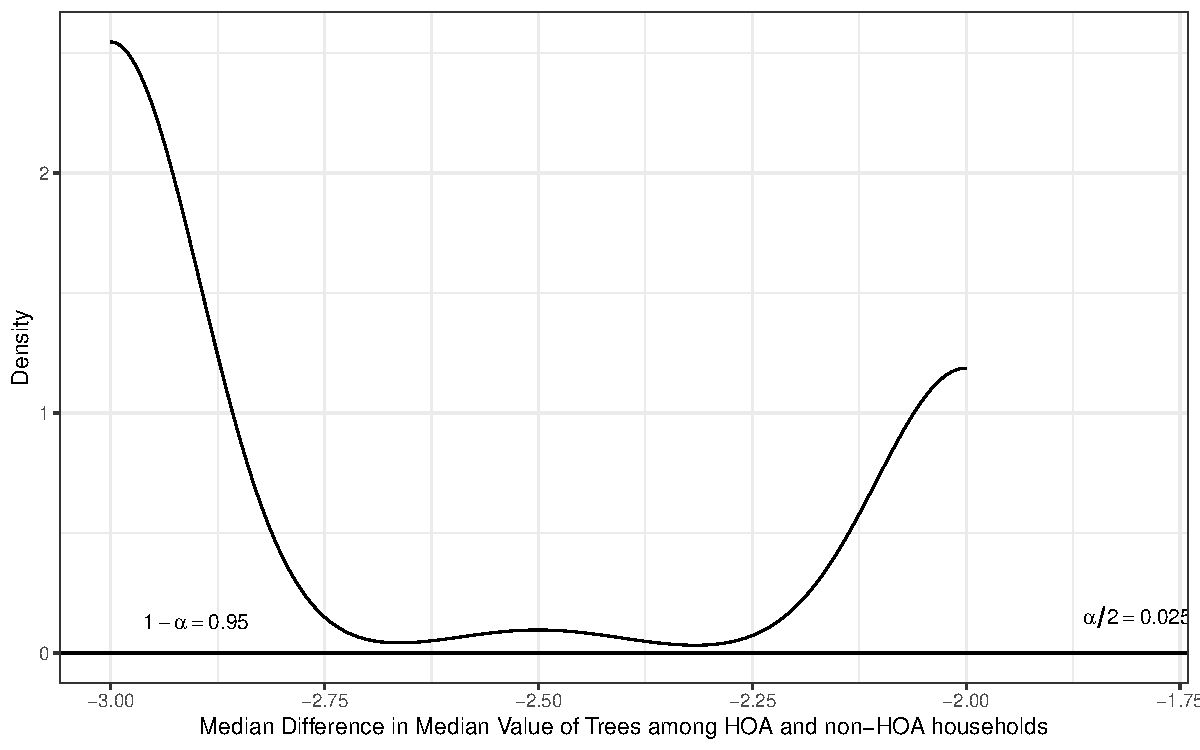
\includegraphics{part2-012}
\caption{The approximate sampling distribution of difference between median number of trees planted by HOA and non-HOA households, with key values of the confidence interval for the population median difference highlighted.} \label{Fig:plot1}
\end{figure}

\textbf{Summarizing analysis}: 

We find statistically significant results to justify our visual analysis that the median number of trees in the front yard of HOA households is lower than those in the front yard of non-HOA households.\\

In other words, we note that the non-HOA households are more sustainable in their tree planting habits relative to HOA households.\\

\textbf{Find in Appendix}: We use the Mood' median test to check if there is a statistically significant difference between the median number of trees planted by HOA and non-HOA households. As expected, the result from Mood's median test may also be used to justify our visual analysis.

\section*{Lawn Care}

\begin{Schunk}
\begin{Sinput}
> LawnCare_summary<-(prop.table(table(dat.HOA$HOA,
+                                     dat.HOA$LawnCare),margin=1))*100
\end{Sinput}
\end{Schunk}

It must be noted that for the purposes of this study, we assume that 4 represents more sustainable behavior than 1 since 1 involves a lot of artificial chemical use. In fact, an increasing order of \textbf{Lawn Care} variable values represents a decreasing order of sustainability behavior among households.

In Table 3, I report a contingency table that documents the percentage of HOA and non-HOA households with Lawn Care values of 1,2,3 and 4. These data are then visualized in Figure 2.

\begin{table}[H]
  \centering
    \begin{tabular}{c|cccc}\hline
    \backslashbox{HOA Status}{Lawn Care} & 1=Excellent & 2=Good & 3=Poor & 4=None \\\hline\hline
    1=Yes & 35.6\% & 23.61\% & 18.32\% & 22.47\%\\
    2=No & 19.75\% & 35.91\% & 32.5\% & 11.85\%\\\hline
    \end{tabular}
    \caption{A contingency table for the HOA status and Lawn Care status of n=1616 observations}
  \end{table}
  
\begin{Schunk}
\begin{Sinput}
> #create ggplot data frame
> tab<-(prop.table(table(dat.HOA$HOA,dat.HOA$LawnCare),margin=1))*100
> xlabs<-c("Excellent","Good","Poor","None")
> ggdat<-data.frame(tab)
> ggplot(data=ggdat,aes(x=Var2,y=Freq,fill=as.factor(Var1)))+
+   geom_bar(stat="identity",
+            position="dodge")+
+   theme_bw()+
+   xlab("Lawn Care Status")+
+   ylab("Proportion (in %) of total households in respective HOA status")+
+   labs(fill = "HOA Status")+
+   ggtitle("Lawn Care by HOA status", 
+   subtitle="Frequencies of Lawn Care by HOA status as a percentage of total number of households in respective HOA
+ status category")+
+   scale_x_discrete(labels=xlabs)+
+   scale_fill_discrete(name="HOA Status", labels= c("Yes", "No"))
\end{Sinput}
\end{Schunk}

\begin{figure}[H]
\centering
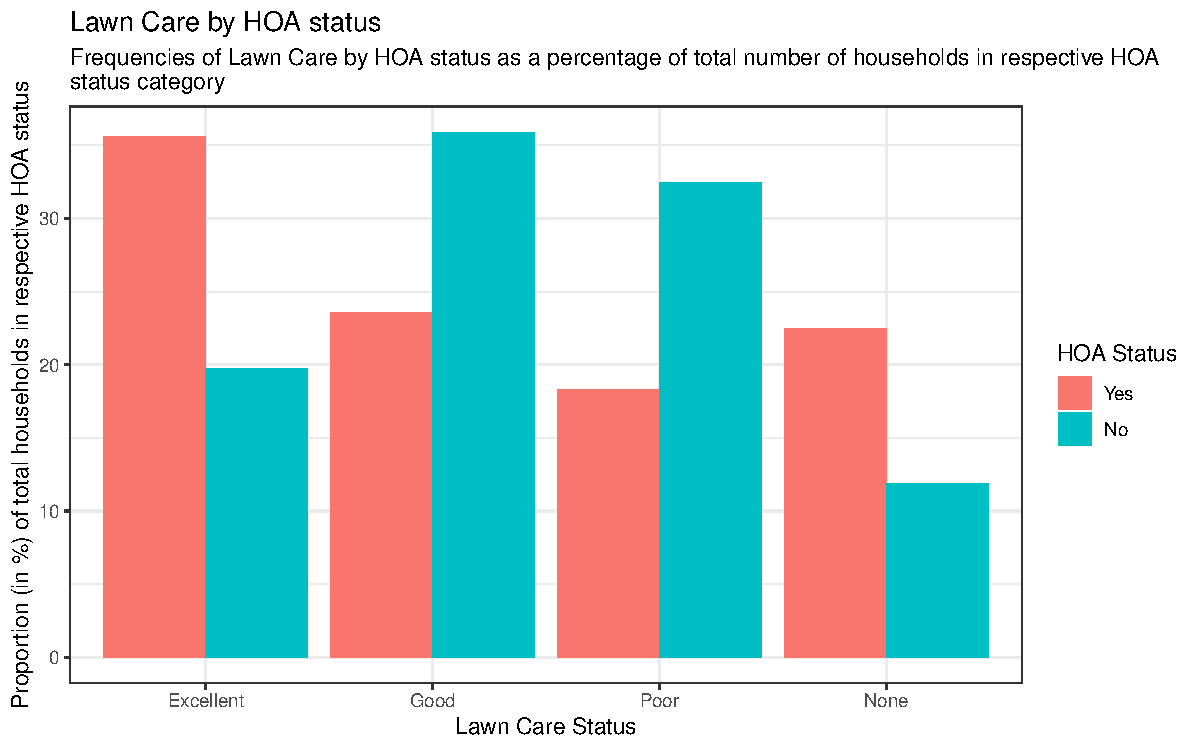
\includegraphics{part2-015}
\caption{Barplot for n=1616 households with 1059 households in HOA and 557 that are not in HOA describing
frequencies of \textbf{Lawn Care} by HOA status of households as a percentage of total number of households in respective HOA status category.} \label{Fig:Plot1}
\end{figure}

\textbf{Visual analysis}:

It is very clear that a very large proportion of HOA households, 35.6\% in magnitude, have Excellent Lawn Care. This is almost double the proportion of non-HOA households that have the same Lawn Care status. In addition, the proportion of HOA households with Good, Poor and None Lawn Care status are almost equal with some amount of variation. For HOA households, then, the analysis of a large number of households with extremely unsustainable behavior that maintain Excellent Lawn Care status is complicated by the realization that there is also a significant number of households engaged in sustainable behavior by having their lawns either naturally managed or managed with low chemical use.\\

For non-HOA households, however, approximately 70\% of the households maintain either Good or Poor Lawn Care status. As a result, relatively few households are engaged in either extremely unsustainable or sustainable behavior in non-HOA households.\\

\textbf{Important takeaway}: Comparing the HOA and non-HOA households, significant differences are noted between the proportion of HOA and non-HOA households maintaining each Lawn Care status category. It seems that the Lawn Care status and HOA status of households are associated with one another, as HOA households are more likely to maintain either Excellent or None lawn care status while non-HOA households are more likely to maintain Good or Poor lawn care status. \\

\textbf{Testing for statistical validity}:

We can use the Chi-squared independence hypothesis test to assess whether or not the two categorical variables of interest to us, Lawn Care status and HOA status of households, are independent. The null and alternate hypotheses for this test are,

$H_{0}$: The Lawn Care status of households is independent of their membership in homeowners' association
$H_{a}$: The Lawn Care status of households is dependent on their membership in homeowners' association

\begin{Schunk}
\begin{Sinput}
> R1<-c(nrow(subset(dat.HOA, dat.HOA$HOA==1 & dat.HOA$LawnCare==1)),
+      nrow(subset(dat.HOA, dat.HOA$HOA==1 & dat.HOA$LawnCare==2)),
+      nrow(subset(dat.HOA, dat.HOA$HOA==1 & dat.HOA$LawnCare==3)),
+      nrow(subset(dat.HOA, dat.HOA$HOA==1 & dat.HOA$LawnCare==4)))
> R2<-c(nrow(subset(dat.HOA, dat.HOA$HOA==2 & dat.HOA$LawnCare==1)),
+      nrow(subset(dat.HOA, dat.HOA$HOA==2 & dat.HOA$LawnCare==2)),
+      nrow(subset(dat.HOA, dat.HOA$HOA==2 & dat.HOA$LawnCare==3)),
+      nrow(subset(dat.HOA, dat.HOA$HOA==2 & dat.HOA$LawnCare==4)))
> LawnCare.tab<-matrix(data=c(R1,R2),
+                  nrow = 2,
+                  ncol = 4,
+                  byrow = TRUE)
> colnames(LawnCare.tab)<-c("Excellent","Good","Poor","None")
> rownames(LawnCare.tab)<-c("Yes","No")
> LawnCare.tab
\end{Sinput}
\begin{Soutput}
    Excellent Good Poor None
Yes       377  250  194  238
No        110  200  181   66
\end{Soutput}
\end{Schunk}

To test these hypotheses using the chi-squared independence hypothesis test we check the assumptions below. \\

1) The two variables are categorical:\\
- Lawn Care Status- Excellent, Good, Poor, None\\
- HOA Status- Yes, No\\

2) Observations are independent\\
- Each household is only reported once\\
- It can be reasonably assumed that observations are independent- a household's outcome doesn't affect another household's outcome\\
- We also assume that the methodology for data collection for this study doesn't introduce any bias\\

3) The sample size is at least the number of cells in the table multiplied by 5;\\
- number of cells x 5= 8 x 5= 40 < 1616.

4) Expected count assumptions are met.

\begin{Schunk}
\begin{Sinput}
> ec_LawnCare<-data.frame()
> for(i in 1:2){
+   counter<-c()
+   for(j in 1:4){
+     counter<-c(counter, (sum(LawnCare.tab[i,])*sum(LawnCare.tab[,j]))/1616)
+   }
+   ec_LawnCare<-rbind(ec_LawnCare, counter)
+ }
> colnames(ec_LawnCare)<-c("Excellent","Good", "Poor", "None")
> rownames(ec_LawnCare)<-c("Yes","No")
> LC<-table(dat.HOA$HOA, dat.HOA$LawnCare)
\end{Sinput}
\end{Schunk}

\begin{table}[H]
  \centering
    \begin{tabular}{c|cccc}\hline
    \backslashbox{HOA Status}{Lawn Care} & Excellent & Good & Poor & None \\\hline\hline
    Yes & 377 (319.14) & 250 (294.89) & 194 (245.75) & 238 (199.22)\\
    No & 110 (167.86) & 200 (155.11) & 181 (129.25) & 66 (104.78)\\\hline
    \end{tabular}
    \caption{A contingency table for the HOA status and Lawn Care status of n=1616 observations (with expected counts for each cell in parentheses)}
  \end{table}

100\% of the expected counts are greater than 5.

The assumptions are met, so we move forward with the test.

% Chi-squared test

\begin{Schunk}
\begin{Sinput}
> chisq.test(LawnCare.tab)
\end{Sinput}
\begin{Soutput}
	Pearson's Chi-squared test

data:  LawnCare.tab
X-squared = 103.78, df = 3, p-value < 2.2e-16
\end{Soutput}
\end{Schunk}

The $p$-value for this test is less than $\alpha= 0.05$. Thus, we reject the null hypothesis. 

We have evidence to suggest that there is a relationship between Lawn Care Status of households and their membership in homeowners' association. We also ask for a confidence interval, via bootstrapping, for the Cramer's association coefficient for the variables Lawn Care Status and HOA status. 

We use the RVAideMemoire (\cite{rvaidememoire}) and the rcompanion (\cite{rcompanion}) packages for this purpose.

\begin{Schunk}
\begin{Sinput}
> library(rcompanion)
> library(RVAideMemoire)
> # cramerV(LawnCare.tab, bias.correct=TRUE)
> cramer.test(LawnCare.tab, conf.level=0.95)
\end{Sinput}
\begin{Soutput}
	Cramér's association coefficient

data:  LawnCare.tab
X-squared = 103.78, df = 3, p-value < 2.2e-16
alternative hypothesis: true association is not equal to 0
95 percent confidence interval:
 0.2100570 0.3012453
sample estimates:
       V 
0.253414 
\end{Soutput}
\end{Schunk}

Here, $k$= min(r,c)= min(2,4)= 2. With respect to the value of $k$, we note that there is little to weak association between Lawn Care Status and HOA status of households. Having noted little to weak association between the two variables of interest, we wish to explore the nature of this association and check our visual analysis on the same above for statistical significance.

In order to numerically verify our insight from visual analysis, we can conduct the z Hypothesis Test to check if there is a statistically significant difference between the proportion of HOA and non-HOA households in each of the 4 Lawn Care status categories.

Before conducting the z Hypothesis tests, we must check the assumptions for the test:\\

1)The sample is generalizable to the population of interest. We assume that the researcher's methodology for collecting data for the study did not introduce any bias. Thus, our samples are generalizable to their respective population HOA and non-HOA households.\\

2) The observations are independent, as no observation affects other observed data. The samples are thus representative of their respective populations.\\

3) The sample sizes $n_{1}$ and $n_{2}$ are reasonably large. We will verify this assumption individually for each hypothesis test.\\

\textbf{Excellent}: Note that $n_{1}$=377 and $n_{2}=110$ here, which are both reasonably large to satisfy the sample size assumption.\\ 

First, we conduct the two sample Z-Hypothesis Test to test the statistical significance of the difference in proportion of HOA and non-HOA households who maintain Excellent Lawn Care status. Following are our hypotheses:\\

$H_{0}: p_{1}-p_{2}= 0$

$H_{a}: p_{1}-p_{2} \neq 0$\\

where, $p_{1}$: Proportion of HOA households who maintain Excellent Lawn Care status

$p_{2}$: Proportion of non-HOA households who maintain Excellent Lawn Care status\\

\begin{Schunk}
\begin{Sinput}
> excellent<-prop.test(x=c(nrow(subset(dat.HOA, 
+         dat.HOA$LawnCare==1 & dat.HOA$HOA==1)),
+         nrow(subset(dat.HOA, dat.HOA$LawnCare==1 & dat.HOA$HOA==2))), 
+         n=c(nrow(subset(dat.HOA, dat.HOA$HOA==1)),
+             nrow(subset(dat.HOA, dat.HOA$HOA==2))), conf.level = 0.95)
> excellent
\end{Sinput}
\begin{Soutput}
	2-sample test for equality of proportions with continuity correction

data:  c(nrow(subset(dat.HOA, dat.HOA$LawnCare == 1 & dat.HOA$HOA ==  out of c(nrow(subset(dat.HOA, dat.HOA$HOA == 1)), nrow(subset(dat.HOA,     1)), nrow(subset(dat.HOA, dat.HOA$LawnCare == 1 & dat.HOA$HOA ==  out of     dat.HOA$HOA == 2)))    2))) out of c(nrow(subset(dat.HOA, dat.HOA$HOA == 1)), nrow(subset(dat.HOA, 
X-squared = 42.81, df = 1, p-value = 6.033e-11
alternative hypothesis: two.sided
95 percent confidence interval:
 0.1132689 0.2037505
sample estimates:
   prop 1    prop 2 
0.3559962 0.1974865 
\end{Soutput}
\end{Schunk}

We note a $p$-value<0.001 which means that we have evidence to conclude that there is a significant difference in the proportion of HOA and non-HOA households who maintain Excellent Lawn Care Status. We also note that the 95\% confidence interval for the difference in population proportions (0.1132, 0.2037) contains only positive values. The numerical evidence, thus, confirms our visual analysis that there is a higher proportion of HOA households who maintain Excellent Lawn Care status as compared to non-HOA households.\\

\textbf{Good}: Note that $n_{1}$=250 and $n_{2}=200$ here, which are both reasonably large to satisfy the sample size assumption.\\

We now conduct the two sample Z-Hypothesis Test to test the statistical significance of the difference in proportion of HOA and non-HOA households who maintain Good Lawn Care status. Following are our hypotheses:

$H_{0}: p_{1}-p_{2}= 0$

$H_{a}: p_{1}-p_{2} \neq 0$\\

where, $p_{1}$: Proportion of HOA households who maintain Good Lawn Care status

$p_{2}$: Proportion of non-HOA households who maintain Good Lawn Care status\\

\begin{Schunk}
\begin{Sinput}
> good<-prop.test(x=c(nrow(subset(dat.HOA, 
+         dat.HOA$LawnCare==2 & dat.HOA$HOA==1)),
+         nrow(subset(dat.HOA, dat.HOA$LawnCare==2 & dat.HOA$HOA==2))), 
+         n=c(nrow(subset(dat.HOA, dat.HOA$HOA==1)),
+             nrow(subset(dat.HOA, dat.HOA$HOA==2))), conf.level = 0.95)
> good
\end{Sinput}
\begin{Soutput}
	2-sample test for equality of proportions with continuity correction

data:  c(nrow(subset(dat.HOA, dat.HOA$LawnCare == 2 & dat.HOA$HOA ==  out of c(nrow(subset(dat.HOA, dat.HOA$HOA == 1)), nrow(subset(dat.HOA,     1)), nrow(subset(dat.HOA, dat.HOA$LawnCare == 2 & dat.HOA$HOA ==  out of     dat.HOA$HOA == 2)))    2))) out of c(nrow(subset(dat.HOA, dat.HOA$HOA == 1)), nrow(subset(dat.HOA, 
X-squared = 26.874, df = 1, p-value = 2.172e-07
alternative hypothesis: two.sided
95 percent confidence interval:
 -0.17170757 -0.07428175
sample estimates:
   prop 1    prop 2 
0.2360718 0.3590664 
\end{Soutput}
\end{Schunk}

We note a $p$-value<0.001 which means that we have evidence to conclude that there is a significant difference in the proportion of HOA and non-HOA households who maintain Good Lawn Care Status. We also note that the 95\% confidence interval for the difference in population proportions (-0.1717, -0.0742) contains only negative values. The numerical evidence, thus, confirms our visual analysis that there is a higher proportion of non-HOA households who maintain Good Lawn Care status as compared to HOA households.\\

\textbf{Poor}: Note that $n_{1}$=194 and $n_{2}=181$ here, which are both reasonably large to satisfy the sample size assumption.\\

We now conduct the two sample Z-Hypothesis Test to test the statistical significance of the difference in proportion of HOA and non-HOA households who maintain Poor Lawn Care status. Following are our hypotheses:

$H_{0}: p_{1}-p_{2}= 0$

$H_{a}: p_{1}-p_{2} \neq 0$\\

where, $p_{1}$: Proportion of HOA households who maintain Poor Lawn Care status

$p_{2}$: Proportion of non-HOA households who maintain Poor Lawn Care status\\

\begin{Schunk}
\begin{Sinput}
> poor<-prop.test(x=c(nrow(subset(dat.HOA, 
+         dat.HOA$LawnCare==3 & dat.HOA$HOA==1)),
+         nrow(subset(dat.HOA, dat.HOA$LawnCare==3 & dat.HOA$HOA==2))), 
+         n=c(nrow(subset(dat.HOA, dat.HOA$HOA==1)),
+             nrow(subset(dat.HOA, dat.HOA$HOA==2))), conf.level = 0.95)
> poor
\end{Sinput}
\begin{Soutput}
	2-sample test for equality of proportions with continuity correction

data:  c(nrow(subset(dat.HOA, dat.HOA$LawnCare == 3 & dat.HOA$HOA ==  out of c(nrow(subset(dat.HOA, dat.HOA$HOA == 1)), nrow(subset(dat.HOA,     1)), nrow(subset(dat.HOA, dat.HOA$LawnCare == 3 & dat.HOA$HOA ==  out of     dat.HOA$HOA == 2)))    2))) out of c(nrow(subset(dat.HOA, dat.HOA$HOA == 1)), nrow(subset(dat.HOA, 
X-squared = 40.372, df = 1, p-value = 2.099e-10
alternative hypothesis: two.sided
95 percent confidence interval:
 -0.18847237 -0.09505449
sample estimates:
   prop 1    prop 2 
0.1831917 0.3249551 
\end{Soutput}
\end{Schunk}

We note a $p$-value<0.001 which means that we have evidence to conclude that there is a significant difference in the proportion of HOA and non-HOA households who maintain Poor Lawn Care Status. We also note that the 95\% confidence interval for the difference in population proportions (-0.1884, -0.0950) contains only negative values. The numerical evidence, thus, confirms our visual analysis that there is a higher proportion of non-HOA households who maintain Poor Lawn Care status as compared to HOA households.

\textbf{None}: Note that $n_{1}$=238 and $n_{2}=66$ here, which are both reasonably large to satisfy the sample size assumption.\\

We now conduct the two sample Z-Hypothesis Test to test the statistical significance of the difference in proportion of HOA and non-HOA households who maintain Poor Lawn Care status. Following are our hypotheses:

$H_{0}: p_{1}-p_{2}= 0$

$H_{a}: p_{1}-p_{2} \neq 0$\\

where, $p_{1}$: Proportion of HOA households who maintain None Lawn Care status

$p_{2}$: Proportion of non-HOA households who maintain None Lawn Care status\\

\begin{Schunk}
\begin{Sinput}
> none<-prop.test(x=c(nrow(subset(dat.HOA, 
+         dat.HOA$LawnCare==4 & dat.HOA$HOA==1)),
+         nrow(subset(dat.HOA, dat.HOA$LawnCare==4 & dat.HOA$HOA==2))), 
+         n=c(nrow(subset(dat.HOA, dat.HOA$HOA==1)),
+             nrow(subset(dat.HOA, dat.HOA$HOA==2))), conf.level = 0.95)
> none
\end{Sinput}
\begin{Soutput}
	2-sample test for equality of proportions with continuity correction

data:  c(nrow(subset(dat.HOA, dat.HOA$LawnCare == 4 & dat.HOA$HOA ==  out of c(nrow(subset(dat.HOA, dat.HOA$HOA == 1)), nrow(subset(dat.HOA,     1)), nrow(subset(dat.HOA, dat.HOA$LawnCare == 4 & dat.HOA$HOA ==  out of     dat.HOA$HOA == 2)))    2))) out of c(nrow(subset(dat.HOA, dat.HOA$HOA == 1)), nrow(subset(dat.HOA, 
X-squared = 26.288, df = 1, p-value = 2.941e-07
alternative hypothesis: two.sided
95 percent confidence interval:
 0.06810377 0.14439303
sample estimates:
   prop 1    prop 2 
0.2247403 0.1184919 
\end{Soutput}
\end{Schunk}

We note a $p$-value<0.001 which means that we have evidence to conclude that there is a significant difference in the proportion of HOA and non-HOA households who maintain Poor Lawn Care Status. We also note that the 95\% confidence interval for the difference in population proportions (0.0681, 0.1443) contains only positive values. The numerical evidence, thus, confirms our visual analysis that there is a higher proportion of HOA households who maintain None Lawn Care status as compared to non-HOA households.\\

\textbf{Summarizing findings:} We conclude that Lawn care status and HOA status of a household have a weak to moderate association. We use the sample data available to visually analyze and confirm, through relevant statistical tests, that HOA households are more likely to maintain Excellent or None lawn care status compared to non-HOA households, while the opposite trend is seen in case of Good and Poor Lawn Care status categories.\\

In other words, HOA households are relatively more likely to have their lawns either highly artificially managed with presumed regular chemical application or have them be fully naturally managed.Thus, HOA households are noted to be either extremely sustainable or extremely unsustainable in the maintenance of their lawns With the evidence available, non-HOA households are relatively more likely to have their lawns be artificially managed at a low to moderate level.\\

Having noted the above, we have inadequate data to declare either group, HOA or non-HOA households, as practicing more sustainable behavior through Lawn care.\\

In order to answer the question, we need data that helps understand if it is better to have a large proportion of households maintain Excellent Lawn Care Status, where the larger proportion still doesn't constitute the majority, as in HOA households, or to have a majority of households maintain moderate chemical use. Such data may result from quantifying the categorical variables for Lawn Care by looking at average chemical use within each category. It must also be noted that answering the question about which sustainability tendency among HOA and non-HOA households is better may also have policy implications, in terms of helping HOA governing or board members identify policies and strategies for promoting more sustainable practices within their neighborhoods.\\

\section*{Garden}

In Table 5, I report a contingency table that documents the percentage of HOA and non-HOA households with and without the presence of a garden in the front or back of their homes. These data are then visualized in Figure 3.

\begin{Schunk}
\begin{Sinput}
> Garden_summary<-(prop.table(table(dat.HOA$HOA,dat.HOA$Garden),margin=1))*100
\end{Sinput}
\end{Schunk}

\begin{table}[H]
  \centering
    \begin{tabular}{c|cc}\hline
    \backslashbox{HOA Status}{Presence of Garden} & Yes & No\\\hline
    Yes & 7.74\% & 92.26\% \\
    No & 10.05\% & 89.95\% \\\hline
    \end{tabular}
    \caption{A contingency table for the HOA status and Garden Presence of n=1616 observations}
  \end{table}
  
\begin{Schunk}
\begin{Sinput}
> #create ggplot data frame
> tab_Garden<-(prop.table(table(dat.HOA$HOA,dat.HOA$Garden),margin=1))*100
> xlabs_Garden<-c("Yes","No")
> ggdat<-data.frame(tab_Garden)
> ggplot(data=ggdat,aes(x=Var2,y=Freq,fill=as.factor(Var1)))+
+   geom_bar(stat="identity",
+            position="dodge")+
+   theme_bw()+
+   xlab("Presence of Garden in the front or back of homes")+
+   ylab("Proportion (in %) of total households in respective HOA status")+
+   labs(fill = "HOA Status")+
+   ggtitle("Presence of Garden by HOA status", 
+           subtitle="Frequencies of Presence of Garden by HOA status as a percentage\nof total number of households in respective HOA status category")+
+   scale_x_discrete(labels=xlabs_Garden)+
+   scale_fill_discrete(name="HOA Status", labels= c("Yes", "No"))
\end{Sinput}
\end{Schunk}

\begin{figure}[H]
\centering
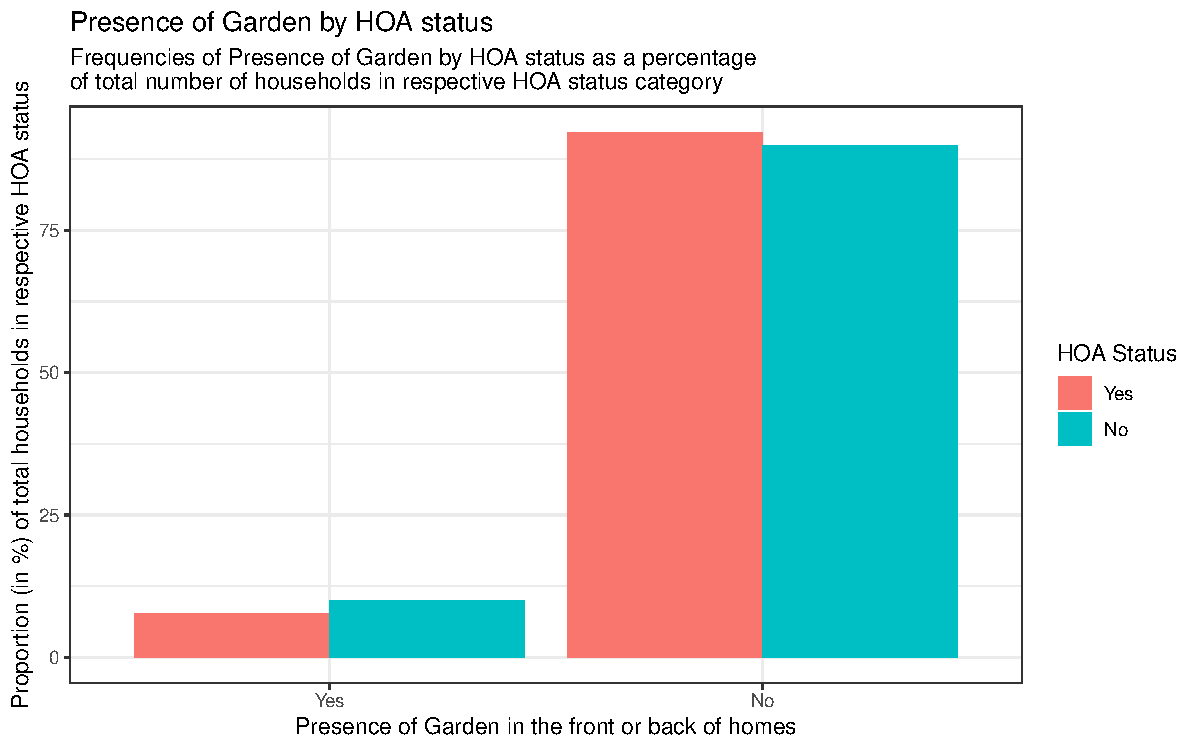
\includegraphics{part2-026}
\caption{Barplot for n=1616 households with 1059 households in HOA and 557 that are not in HOA describing
frequencies of \textbf{Presence of Garden} by HOA status of households as a percentage of total number of households in respective HOA status category.} \label{Fig:Plot1}
\end{figure}

\textbf{Visual analysis}:

It seems that there is relatively little difference in home gardening tendencies between HOA and non-HOA households. Even though the proportion of non-HOA households who have a garden is slightly higher than the proportion of HOA households who have a garden, a very high proportion of both HOA and non-HOA households do not have a garden. Numerically, approximately 92\% of HOA households and 90\% of non-HOA households do not have a garden.\\

\textbf{Testing for statistical significance}:

We can use the Chi-Squared Independence Test to assess whether or not the two categorical variables of interest to us, presence of garden in homes and HOA status of households, are independent. Note that even though we may use the Fisher's Exact Test because both of our categorical variables have only two observable values (Yes, No), we avoid doing so because our sample size of 1616 households, 1059 of which are members of homeowners' association while 557 are not, seems pretty large for Fisher's Exact Test which is typically used for small-sample tests. The null and alternate hypotheses for this test are:\\

$H_{0}$: The presence of garden in households is independent of their membership in homeowners' association 

$H_{a}$: The presence of garden in households is dependent on their membership in homeowners' association

\begin{Schunk}
\begin{Sinput}
> O11<-nrow(subset(dat.HOA, dat.HOA$HOA==1 & dat.HOA$Garden==1))
> O12<-nrow(subset(dat.HOA, dat.HOA$HOA==1 & dat.HOA$Garden==2))
> O21<-nrow(subset(dat.HOA, dat.HOA$HOA==2 & dat.HOA$Garden==1))
> O22<-nrow(subset(dat.HOA, dat.HOA$HOA==2 & dat.HOA$Garden==2))
> Garden.tab<-matrix(data=c(O11,O12,O21,O22),
+                 nrow = 2,
+                 ncol = 2,
+                 byrow = TRUE)
> colnames(Garden.tab)<-c("Yes","No")
> rownames(Garden.tab)<-c("Yes","No")
> Garden.tab
\end{Sinput}
\begin{Soutput}
    Yes  No
Yes  82 977
No   56 501
\end{Soutput}
\end{Schunk}

To test these hypotheses using Chi-Squared Independence Test, we first check the assumptions of the test:\\

1) The two variables are categorical.\\
- Garden presence: Yes or No\\
- HOA status: Yes or No\\

2) The observations are independent\\
- It can be reasonably assumed that observations are independent- one observation's outcomes, whether in terms of HOA status or garden presence or any other variable of interest, doesn't affect later observations.\\
- Each sample can be represented in one and only one cell of the table.\\

3) The sample size is at least the number of cells in the table multiplied by 5;\\
- number of cells x 5= 4 x 5= 20 < 1616.\\

4) Expected count assumptions are met.

\begin{Schunk}
\begin{Sinput}
> ec_Garden<-data.frame()
> for(i in 1:2){
+   counter<-c()
+   for(j in 1:2){
+     counter<-c(counter, (sum(Garden.tab[i,])*sum(Garden.tab[,j]))/1616)
+   }
+   ec_Garden<-rbind(ec_Garden, counter)
+ }
> colnames(ec_Garden)<-c("Yes","No")
> rownames(ec_Garden)<-c("Yes","No")
\end{Sinput}
\end{Schunk}

\begin{table}[H]
  \centering
    \begin{tabular}{c|cc}\hline
    \backslashbox{HOA Status}{Presence of Garden} & Yes & No\\\hline
    Yes & 82 (90.43) & 977 (968.57) \\
    No & 56 (47.57) & 501 (509.43) \\\hline
    \end{tabular}
    \caption{A contingency table for the HOA status and Garden Presence of n=1616 observations (with expected counts for each cell in parentheses)}
  \end{table}

100\% of the expected counts are greater than 5.\\

The assumptions are met, so we move forward with the test.\\

% Chi-squared Test

\begin{Schunk}
\begin{Sinput}
> chisq.test(Garden.tab) # not significant
\end{Sinput}
\begin{Soutput}
	Pearson's Chi-squared test with Yates' continuity correction

data:  Garden.tab
X-squared = 2.2082, df = 1, p-value = 0.1373
\end{Soutput}
\end{Schunk}

The p-value for this test is 0.1373, which is less than $\alpha$ equal to 0.05. Thus, we fail to reject the null hypothesis.\\

Thus, we do not have evidence to suggest that there is a statistically significant relationship between Lawn Care Status of households and their membership in homeowners' association.\\

\textbf{Summarizing analysis}: After visually analyzing the barplot in Figure 3, we suspected little difference in home gardening tendencies across the two HOA status categories. However, we found a small negative difference between the proportion of HOA and non-HOA households who had a garden, and wanted to check if this difference was statistically significant.\\

Applying the Chi-squared hypothesis test, we fail to find evidence of any association between garden presence and HOA status of households, which supports our visual analysis. The sample data, thus, suggests a general lack of home gardening tendency at the homeowner level, irrespective of HOA status of households.\\

\textbf{An important note}: Home gardening has often been associated with the maintenance of ecological, economic and social sustainability of these homes. In fact, home gardens also play a key role in maintaining the biological diversity of native and exotic as well as managed or wild species and in improving the quality of life for members residing in these households, according to recent research on home gardens as alternatives for sustainability with a special emphasis on Latin America (\cite{homegarden}). If this sample is a representative sample of a larger population, the lack of home gardening tendencies, regardless of HOA status of households, may be concerning.\\

\section*{Recycling}

In Table 7, I report a contingency table that documents the percentage of HOA and non-HOA households with the recycling status of these households. These data are then visualized in Figure 6.

\begin{Schunk}
\begin{Sinput}
> Recycling_summary<-(prop.table(table(dat.HOA$HOA,dat.HOA$Recycle),margin=1))*100
\end{Sinput}
\end{Schunk}

\begin{table}[H]
  \centering
    \begin{tabular}{c|ccc}\hline
    \backslashbox{HOA Status}{Recycling Status} 
    &$\begin{matrix} \text{Recycling and trash}\\ \text{bins present at home} \end{matrix} $
    & $\begin{matrix} \text{Only trash bin}\\ \text{present} \end{matrix}$ 
    & $\begin{matrix} \text{Recycling bin status unobservable}\\ \text{under method of data collection}
    \\ \text{(no curb-side pickup)} \end{matrix}$ \\\hline
    Yes & 57.98\% & 21.72\% & 
    20.3\%\\
    No & 66.97\% & 22.44\% & 
    10.59\%\\\hline
    \end{tabular}
    \caption{A contingency table for the HOA status and Recycling status of n=1616 observations}
  \end{table}
  
\begin{Schunk}
\begin{Sinput}
> #create ggplot data frame
> tab_Recycle<-(prop.table(table(dat.HOA$HOA,dat.HOA$Recycle),margin=1))*100
> xlabs_Recycle<-c("Recycle bin and trash bin present",
+                  "Only trash bin present", 
+                  "Unobservable (no curb sise pick-up)")
> ggdat<-data.frame(tab_Recycle)
> ggplot(data=ggdat,aes(x=Var2,y=Freq,fill=as.factor(Var1)))+
+   geom_bar(stat="identity",
+            position="dodge")+
+   theme_bw()+
+   xlab("Recycling Status of households")+
+   ylab("Proportion (in %) of total households in respective HOA status")+
+   labs(fill = "HOA Status")+
+   ggtitle("Recycling status by membership in HOA", 
+           subtitle="Frequencies of Recycling Status by HOA status as a percentage of total number of households in \nrespective HOA status category")+
+   scale_x_discrete(labels=xlabs_Recycle)+
+   scale_fill_discrete(name="HOA Status", labels= c("Yes", "No"))
\end{Sinput}
\end{Schunk}

\begin{figure}[H]
\centering
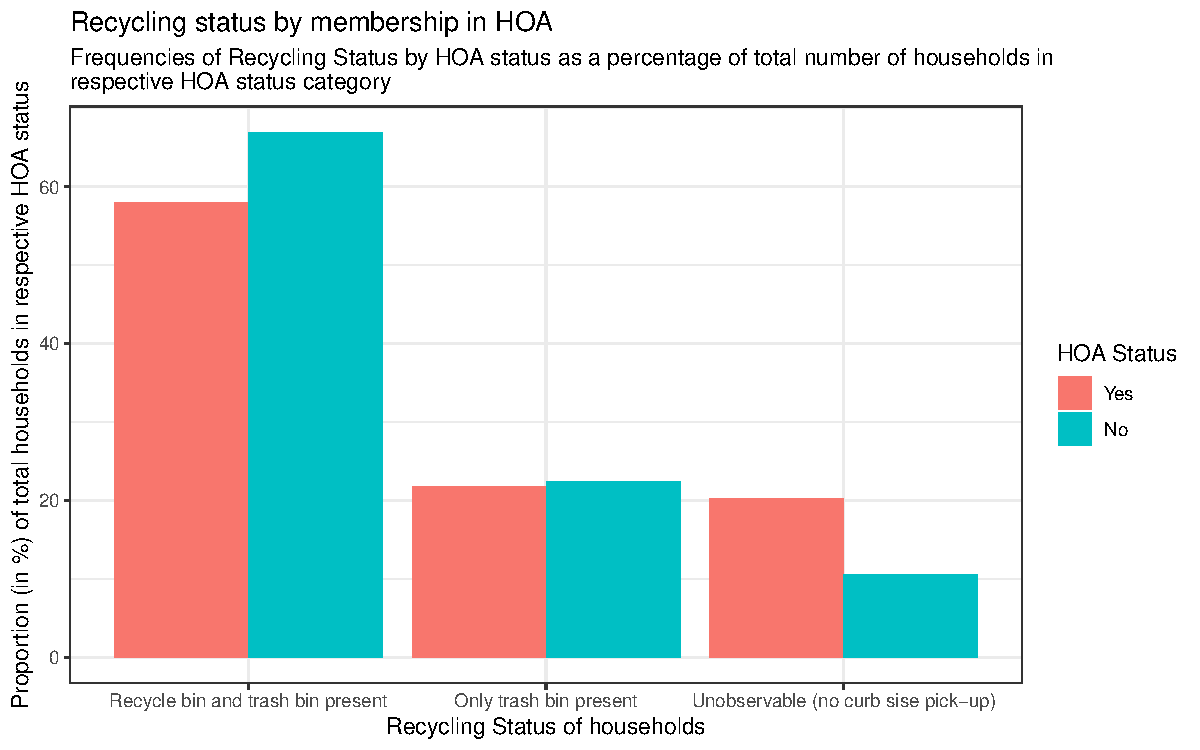
\includegraphics{part2-032}
\caption{Bar plot for n=1616 households with 1059 households in HOA and 557 that are not in HOA describing
frequencies of \textbf{Recycling status} by HOA status of households as a percentage of total number of households in respective HOA status category.} \label{Fig:Plot1}
\end{figure}

\textbf{Visual Analysis:} 

The proportion of households who have a recycling bin at their homes is higher for non-HOA households, as compared to HOA households, by a seemingly significant or non-trivial difference while the proportion of households which only have a trash bin is almost equal across both HOA status. In addition, it must also be noted that the proportion of households with unobservable values of recycling status for HOA households is almost double that of non-HOA households.\\

Just visually analyzing the barplot in Figure 6, overall, we note three main insights. 

1) There is extremely little difference between the proportion of HOA and non-HOA households which have only a trash bin present. \\

2) It seems that non-HOA households are relatively more likely to have a recycling bin present. \\

3) The sample data suggests HOA households are relatively less likely to have curb side pickup within their neighborhoods.\\

So, we find visual evidence that non-HOA households have relatively better recycling habits, in terms of the presence of a recycling bin, compared to HOA households within the limitations of the data available. However, we aim to fully explore the large proportion of HOA households with unobservable values of recycling status through statistical tests and understand its implications on the larger research question.\\

\textbf{Statistical tests}:

We can use the Chi-squared independence hypothesis test to assess whether or not the two categorical variables of interest to us, Recycling status and HOA status of households, are independent. The null and alternate hypotheses for this test are:\\

$H_{0}$: The Recycling status of households is independent of their membership in homeowners' association

$H_{a}$: The Recycling status of households is dependent on their membership in homeowners' association\\

% Chi-squared test- with 3 categories for Recycling

\begin{Schunk}
\begin{Sinput}
> R1<-c(nrow(subset(dat.HOA, dat.HOA$HOA==1 & dat.HOA$Recycle==1)),
+      nrow(subset(dat.HOA, dat.HOA$HOA==1 & dat.HOA$Recycle==2)),
+      nrow(subset(dat.HOA, dat.HOA$HOA==1 & dat.HOA$Recycle==3)))
> R2<-c(nrow(subset(dat.HOA, dat.HOA$HOA==2 & dat.HOA$Recycle==1)),
+      nrow(subset(dat.HOA, dat.HOA$HOA==2 & dat.HOA$Recycle==2)),
+      nrow(subset(dat.HOA, dat.HOA$HOA==2 & dat.HOA$Recycle==3)))
> Recycle.tab<-matrix(data=c(R1,R2),
+                  nrow = 2,
+                  ncol = 3,
+                  byrow = TRUE)
> colnames(Recycle.tab)<-c("Recycling and trash bin","Only trash bin","Recycling status unobservable")
> rownames(Recycle.tab)<-c("Yes","No")
> Recycle.tab
\end{Sinput}
\begin{Soutput}
    Recycling and trash bin Only trash bin Recycling status unobservable
Yes                     614            230                           215
No                      373            125                            59
\end{Soutput}
\end{Schunk}

To test these hypotheses using the chi-squared independence hypothesis test we check the assumptions below. \\

1) The two variables are categorical:\\
- Recycling Status- Both Recycling bin and trash bin present at the home, Only a trash bin was present, Recycling status unobservable under method of data collection (no curb-side pickup)\\
- HOA Status- Yes, No\\

2) Observations are independent\\
- Each household is only reported once\\
- It can be reasonably assumed that observations are independent- a household's outcome doesn't affect another household's outcome\\
- We also assume that the methodology for data collection for this study doesn't introduce any bias\\

3) The sample size is at least the number of cells in the table multiplied by 5;\\
- number of cells x 5= 6 x 5= 30 < 1616.

4) Expected count assumptions are met.

\begin{Schunk}
\begin{Sinput}
> ec_Recycle<-data.frame()
> for(i in 1:2){
+   counter<-c()
+   for(j in 1:3){
+     counter<-c(counter, (sum(Recycle.tab[i,])*sum(Recycle.tab[,j]))/1616)
+   }
+   ec_Recycle<-rbind(ec_Recycle, counter)
+ }
> colnames(ec_Recycle)<-c("Recycling and trash bin","Only trash bin","Recycling status unobservable")
> rownames(ec_Recycle)<-c("Yes","No")
\end{Sinput}
\end{Schunk}

\begin{table}[H]
  \centering
    \begin{tabular}{c|ccc}\hline
    \backslashbox{HOA Status}{Recycling Status} 
    &$\begin{matrix} \text{Recycling and trash}\\ \text{bins present at home} \end{matrix} $
    & $\begin{matrix} \text{Only trash bin}\\ \text{present} \end{matrix}$ 
    & $\begin{matrix} \text{Recycling bin status unobservable}\\ \text{under method of data collection}
    \\ \text{(no curb-side pickup)} \end{matrix}$ \\\hline
    Yes & 614 (646.8) & 230 (232.64) & 
    215 (179.56)\\
    No & 373 (340.2) & 125 (122.36) & 
    59 (94.44)\\\hline
    \end{tabular}
    \caption{A contingency table for the HOA status and Recycling status of n=1616 observations (with expected value for each cell in parentheses)}
  \end{table}

100\% of the expected counts are greater than 5.

The assumptions are met, so we move forward with the test.

\begin{Schunk}
\begin{Sinput}
> chisq.test(Recycle.tab) # significant
\end{Sinput}
\begin{Soutput}
	Pearson's Chi-squared test

data:  Recycle.tab
X-squared = 25.209, df = 2, p-value = 3.356e-06
\end{Soutput}
\end{Schunk}

The p-value for this test is less than $\alpha= 0.05$. Thus, we reject the null hypothesis. \\

We have evidence to suggest that there is a relationship between Recycling Status of households and their membership in homeowners' association. We also ask for a confidence interval, via bootstrapping, for the Cramer's association coefficient for the variables Lawn Care Status and HOA status. 

\begin{Schunk}
\begin{Sinput}
> library(rcompanion)
> library(RVAideMemoire)
> # cramerV(Recycle.tab, bias.correct=TRUE)
> cramer.test(Recycle.tab, conf.level=0.95)
\end{Sinput}
\begin{Soutput}
	Cramér's association coefficient

data:  Recycle.tab
X-squared = 25.209, df = 2, p-value = 3.356e-06
alternative hypothesis: true association is not equal to 0
95 percent confidence interval:
 0.08722848 0.17040808
sample estimates:
        V 
0.1248997 
\end{Soutput}
\end{Schunk}

Here, $k$= min(r,c)= min(2,3)= 2. With respect to the value of $k$, we note that there is little to weak association between Lawn Care Status and HOA status of households. Having noted a little to weak association among the two variables of interest, we wish to use statistical tests to verify the nature of the association that we predicted in our visual analysis above.\\

In order to numerically test the statistical validity of our second and third visual visual insights noted above, we shall conduct two sample Z-hypothesis tests. Before conducting the z Hypothesis tests, we must check the assumptions for the test:\\

1)The sample is generalizable to the population of interest. We assume that the researcher's methodology for collecting data for the study did not introduce any bias. Thus, our samples are generalizable to their respective population HOA and non-HOA households.

2) The observations are independent, as no observation affects other observed data. The samples are thus representative of their respective populations.

3) The sample sizes $n_{1}$ and $n_{2}$ are reasonably large.\\

1) The proportion of HOA and non-HOA households which have both recycling and trash bin present\\

First, we conduct the two sample Z-Hypothesis Test to test the statistical significance of the difference in proportion of HOA and non-HOA households who maintain Excellent Lawn Care status. Following are our hypotheses:

$H_{0}: p_{1}-p_{2}= 0$

$H_{a}: p_{1}-p_{2} \neq 0$\\

where, $p_{1}$: Proportion of HOA households which have both recycling and trash bin present

$p_{2}$: Proportion of non-HOA households which have both recycling and trash bin present\\

\begin{Schunk}
\begin{Sinput}
> RecyclingBin<-prop.test(x=c(nrow(subset(dat.HOA, 
+         dat.HOA$Recycle==1 & dat.HOA$HOA==1)),
+         nrow(subset(dat.HOA, dat.HOA$Recycle==1 & dat.HOA$HOA==2))), 
+         n=c(nrow(subset(dat.HOA, dat.HOA$HOA==1)),
+             nrow(subset(dat.HOA, dat.HOA$HOA==2))), conf.level = 0.95)
> RecyclingBin
\end{Sinput}
\begin{Soutput}
	2-sample test for equality of proportions with continuity correction

data:  c(nrow(subset(dat.HOA, dat.HOA$Recycle == 1 & dat.HOA$HOA ==  out of c(nrow(subset(dat.HOA, dat.HOA$HOA == 1)), nrow(subset(dat.HOA,     1)), nrow(subset(dat.HOA, dat.HOA$Recycle == 1 & dat.HOA$HOA ==  out of     dat.HOA$HOA == 2)))    2))) out of c(nrow(subset(dat.HOA, dat.HOA$HOA == 1)), nrow(subset(dat.HOA, 
X-squared = 12.025, df = 1, p-value = 0.000525
alternative hypothesis: two.sided
95 percent confidence interval:
 -0.14032231 -0.03941095
sample estimates:
   prop 1    prop 2 
0.5797923 0.6696589 
\end{Soutput}
\end{Schunk}

We note a $p$-value= 0.000525, which is less than $\alpha$=0.05. Thus, we have evidence to conclude that there is a significant difference in the proportion of HOA and non-HOA households which have both recycling and trash bin present. We also note that the 95\% confidence interval for the difference in population proportions (-0.1403, -0.0394) contains only negative values. The numerical evidence, thus, confirms our visual analysis that non-HOA households are relatively more likely to have both recycling and trash bin present.\\

2) The proportion of HOA and non-HOA households with no curb-side pickup within their neighborhoods\\

We conduct the two sample Z-Hypothesis Test to test the statistical significance of the difference in proportion of HOA and non-HOA households associated with neighborhoods having no curb side pickup. Following are our hypotheses:

$H_{0}: p_{1}-p_{2}= 0$

$H_{a}: p_{1}-p_{2} \neq 0$\\

where, $p_{1}$: Proportion of HOA households associated with neighborhoods having no curb side pickup

$p_{2}$: Proportion of non-HOA households associated with neighborhoods having no curb side pickup\\

\begin{Schunk}
\begin{Sinput}
> CurbPickup<-prop.test(x=c(nrow(subset(dat.HOA, 
+         dat.HOA$Recycle==3 & dat.HOA$HOA==1)),
+         nrow(subset(dat.HOA, dat.HOA$Recycle==3 & dat.HOA$HOA==2))), 
+         n=c(nrow(subset(dat.HOA, dat.HOA$HOA==1)),
+             nrow(subset(dat.HOA, dat.HOA$HOA==2))), conf.level = 0.95)
> CurbPickup
\end{Sinput}
\begin{Soutput}
	2-sample test for equality of proportions with continuity correction

data:  c(nrow(subset(dat.HOA, dat.HOA$Recycle == 3 & dat.HOA$HOA ==  out of c(nrow(subset(dat.HOA, dat.HOA$HOA == 1)), nrow(subset(dat.HOA,     1)), nrow(subset(dat.HOA, dat.HOA$Recycle == 3 & dat.HOA$HOA ==  out of     dat.HOA$HOA == 2)))    2))) out of c(nrow(subset(dat.HOA, dat.HOA$HOA == 1)), nrow(subset(dat.HOA, 
X-squared = 23.755, df = 1, p-value = 1.094e-06
alternative hypothesis: two.sided
95 percent confidence interval:
 0.06051251 0.13368174
sample estimates:
   prop 1    prop 2 
0.2030217 0.1059246 
\end{Soutput}
\end{Schunk}

We note a p-value<0.01. Thus. we have evidence to conclude that there is a statistically significant difference between the proportion of HOA and non-HOA households which are associated with neighborhoods with no curb side pickup.  We also note that the 95\% confidence interval for the difference in proportions only includes positive values. The numerical result confirms our visual analysis that HOA households are relatively less likely to have curb side pickup in their respective neighborhoods.\\

\textbf{Summarizing analysis}: We find little to weak association between the variables Recycling status of households and HOA status of households. The numerical results confirm our visual analysis that non-HOA households are relatively more likely to have both trash and recycling bin present, and HOA households are more likely to be in neighborhoods with no curb side pickup.\\

Thus, we find evidence that non-HOA households are relatively more sustainable in their recycling habits. We note that the relatively better recycling habits among non-HOA households may also result, to a questionable degree of extent, from their relatively higher presence in neighborhoods with curb side pickup. The data, thus, suggests that a difference in recycling habits between HOA and non-HOA households doesn't merely reflect a difference in homeowner behavior. It also reflects the impact of differences in relative distribution of HOA and non-HOA households across different neighborhoods, with varying amenities like curb-side pickup, on the sustainability outcomes of these households.\\

\section*{Comparing individual sustainability indicators between neighborhoods with HOAs and those without: an overall assessment}

Overall, I am inclined to say that non-HOA households show relatively better sustainablity habits and tendencies, as compared to those of HOA households. Following is a brief justification that ties back all analysis until this point: \\

\textbf{Trees}: We find evidence that the median number of trees planted by non-HOA households is greater than the median number of trees planted by HOA households. We note that non-HOA households are clearly more sustainable in their tree planting habits by virtue of a relatively higher number of trees planted.\\

\textbf{Recycling}: We find evidence that non-HOA households are relatively more likely to have a recycling bin present. However, we also found evidence that non-HOA households are relatively more likely to be in a neighborhood with curb-side pickup.Thus, non-HOA households having relatively better recycling tendencies may be a reflection of either better homeowner behavior or access to curb side pickup facilities. 

Within the limitations of the data, however, we note that non-HOA households are relatively more sustainable in their recycling habits.\\

\textbf{Garden presence}: We concluded that the presence of a garden in a household is independent of its HOA status.\\

\textbf{Lawn Care}: We noted that HOA households are more likely to have their lawns fully artificially or fully naturally managed, while non-HOA households are more likely to use little to moderate chemicals to manage their lawns. We do not have the technical expertise or the data to declare either HOA or non-HOA households as having more sustainable Lawn Care habits.\\

Even though we fail to determine HOA or non-HOA households as being more sustainable specifically in terms of Garden presence and Lawn care sustainability indicators, we note that relatively better recycling and tree planting tendencies among non-HOA households is sufficient justification to support our overall assessment.\\

\section*{Relationship among multiple sustainability indicators}

\section*{Relationship between Recycling tendency and Lawn Care Status of households}

Table 9 below analyzes the frequencies of Lawn Care status by Recycling status separately for HOA and non-HOA households. Note that separating the analysis for HOA and non-HOA households allows us to add specificity to our analysis and helps us discover trends that may be specific to an HOA category but may be lost in generalizing to the entire sample data.

\begin{Schunk}
\begin{Sinput}
> RLC<-(prop.table(table(subset(dat.HOA, dat.HOA$HOA==1)$Recycle,
+                         subset(dat.HOA, dat.HOA$HOA==1)$LawnCare),margin=1))*100
> RLC2<-(prop.table(table(subset(dat.HOA, dat.HOA$HOA==2)$Recycle,
+                         subset(dat.HOA, dat.HOA$HOA==2)$LawnCare),margin=1))*100
\end{Sinput}
\end{Schunk}

% Recycling Status and Lawn Care
\begin{table}[H]
  \centering
    \begin{tabular}{|c|c|c|c|c|c|}\hline
    HOA &
    \backslashbox{Recycling Status}{Lawn Care Status} 
    & Excellent & Good & Poor & None \\\hline\hline
    
    & $\begin{matrix} \text{Recycling and trash}\\ \text{bins present at home} \end{matrix}$ &
    38.76\% & 24.27\% & 
    17.26\% & 
    19.71\%\\\hline\hline
    
    Yes & $\begin{matrix} \text{Only trash bin}\\ \text{present} \end{matrix}$ &
    24.35\% & 20.87\% & 
    23.91\% & 
    30.87\%\\\hline\hline
    
    & $\begin{matrix} \text{Unobservable Recycling status}\\ \end{matrix}$ &
    38.6\% & 24.65\% & 
    15.35\% & 
    21.4\%\\\hline\hline
    
    & $\begin{matrix} \text{Recycling and trash}\\ \text{bins present at home} \end{matrix}$ &
    21.98\% & 34.58\% & 
    31.9\% & 
    11.53\%\\\hline\hline
    
    No & $\begin{matrix} \text{Only trash bin}\\ \text{present} \end{matrix}$ &
    12.8\% & 41.6\% & 
    35.2\% & 
    10.4\%\\\hline\hline
    
    & $\begin{matrix} \text{Unobservable Recycling status}\\ \end{matrix}$ &
    20.34\% & 32.2\% & 
    30.51\% & 
    16.95\%\\\hline\hline
    
    \end{tabular}
    \caption{A contingency table for the Recycling Status and Lawn Care status of n=1616 observations categorized separately by HOA status}
  \end{table}
  
We visualize the data in Table 9 in Figure 6. 

Here, we use the clauscowplot package (\cite{clauscowplot}).

\begin{Schunk}
\begin{Sinput}
> #create ggplot data frame
> library("cowplot")
> tab_LawnCareRecycle<-(prop.table(table(subset(dat.HOA, dat.HOA$HOA==1)$Recycle,
+                                        subset(dat.HOA, dat.HOA$HOA==1)$LawnCare),
+                                  margin=1))*100
> xlabs_LawnCareRecycle<-c("Excellent","Good","Poor","None")
> ggdat<-data.frame(tab_LawnCareRecycle)
> p1<-ggplot(data=ggdat,aes(x=Var2,y=Freq,fill=as.factor(Var1)))+
+   geom_bar(stat="identity",
+            position="dodge")+
+   theme_bw()+
+   xlab("Lawn Care Status")+
+   ylab("Proportion (in %) of total HOA households\nin respective recycling status")+
+   scale_fill_discrete(name="Recycling Status", labels= 
+                         c("Recycle bin and trash bin present",
+                           "Only trash bin present", 
+                           "Unobservable (no curb sise pick-up)"))+
+   ggtitle("Lawn Care status by Recycling status for\nonly 
+           HOA households (HOA=1)", subtitle="Frequencies of Lawn Care Status by 
+           Recycling\nstatus for households with HOA=1")+
+   scale_x_discrete(labels=xlabs_LawnCareRecycle)+
+   theme(legend.position = "bottom", legend.direction = "vertical")+
+   theme(plot.margin = unit(c(1, 1, 1, 0), "lines"))
> tab_LawnCareRecycle<-(prop.table(table(subset(dat.HOA, dat.HOA$HOA==2)$Recycle,
+                                        subset(dat.HOA, dat.HOA$HOA==2)$LawnCare),margin=1))*100
> xlabs_LawnCareRecycle<-c("Excellent","Good","Poor","None")
> ggdat<-data.frame(tab_LawnCareRecycle)
> p2<-ggplot(data=ggdat,aes(x=Var2,y=Freq,fill=as.factor(Var1)))+
+   geom_bar(stat="identity",
+            position="dodge")+
+   theme_bw()+
+   xlab("Lawn Care Status")+
+   ylab("Proportion (in %) of total non-HOA households\nin respective 
+        recycling status")+
+   scale_fill_discrete(name="Recycling Status", labels= c("Recycle bin 
+                                                          and trash bin present",
+                                                          "Only trash bin present", 
+                                                          "Unobservable 
+                                                          (no curb sise pick-up)"))+
+   ggtitle("Lawn Care status by Recycling status for\nonly non-HOA households (HOA=2)",
+           subtitle="Frequencies of Lawn Care Status by Recycling\nstatus for 
+           non-HOA households with HOA=2")+
+   scale_x_discrete(labels=xlabs_LawnCareRecycle)+
+   theme(legend.position = "bottom", legend.direction = "vertical")+
+   theme(plot.margin = unit(c(1, 1, 1, 1), "lines"))
> grid.arrange(p1,p2,ncol=2)
\end{Sinput}
\end{Schunk}

\begin{figure}[H]
\centering
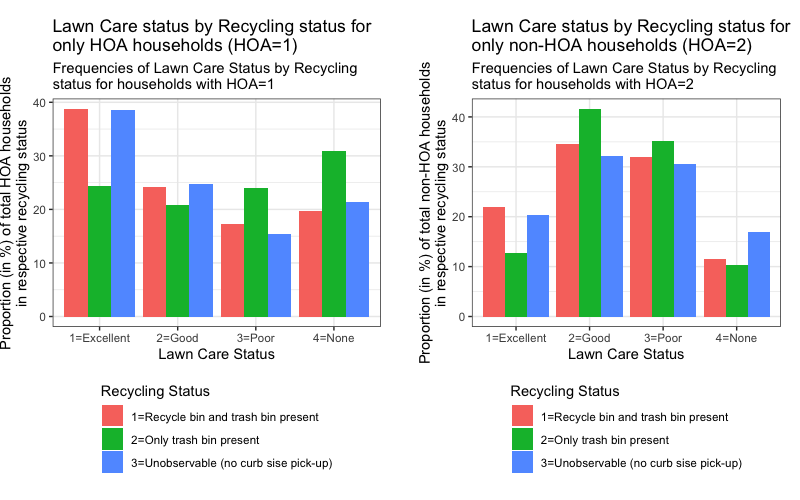
\includegraphics[scale=2]{LawnCareRecycle.png}
\caption{Barplot for n=1616 households with 1059 households in HOA describing frequencies of \textbf{LawnCare status} by Recycling status of households as a percentage of total number of households in respective Recycling status category for a particular HOA category. \textbf{Left:} Only HOA households \textbf{Right:} Only non-HOA households} \label{Fig:Plot1}
\end{figure}

\textbf{Visual analysis}:

We notice that for HOA households, there is a noticeable relationship between Recycling status and Lawn Care status. Essentially, there is a very high proportion of HOA households that recycle and maintain Excellent Lawn Care. The proportion of households decreases almost consistently within categories of increasing Lawn Care status for all households that recycle.\\

Again, the majority of HOA households who don't recycle are concentrated within Poor and None Lawn Care status. To a great extent, better recycling tendencies are linked to more unsustainable Lawn Care status within HOA households.\\

Such a clear relationship between Lawn Care status and Recycling tendency is not noted in case of non-HOA households. Regardless of the Recycling status of non-HOA households, the distribution of proportion of non-HOA households within different Lawn Care status is almost the same with the majority of households concentrated in Good and Poor Lawn Care status.\\

Visually, we notice that there is some association between Lawn Care status and Recycling status within HOA households. However, no noticeable association or clear relationship between the two variables is seen in case of non-HOA households.\\

\textbf{Statistical tests}:

We will use the Chi-square independence hypothesis test to assess whether there is a statistically significant association between the variables Recycling and Lawn Care Status. We shall be using this test separately for HOA and non-HOA households.

\textbf{HOA households}:

We first use the Chi-squared independence hypothesis test to test the following hypothesis for HOA households:\\

$H_{0}$: The Lawn Care status of HOA households is independent of their Recycling Status 

$H_{a}$: The Lawn Care status of HOA households is dependent on their Recycling status\\

\begin{Schunk}
\begin{Sinput}
> R1<-c(nrow(subset(dat.HOA, dat.HOA$HOA==1 & dat.HOA$Recycle==1 
+     & dat.HOA$LawnCare==1)), 
+     nrow(subset(dat.HOA, dat.HOA$HOA==1 
+     & dat.HOA$Recycle==1 & dat.HOA$LawnCare==2)), 
+     nrow(subset(dat.HOA, dat.HOA$HOA==1 & dat.HOA$Recycle==1 
+     & dat.HOA$LawnCare==3)),
+     nrow(subset(dat.HOA, dat.HOA$HOA==1 & dat.HOA$Recycle==1 & 
+     dat.HOA$LawnCare==4)))
> R2<-c(nrow(subset(dat.HOA, dat.HOA$HOA==1 & dat.HOA$Recycle==2 
+     & dat.HOA$LawnCare==1)), 
+     nrow(subset(dat.HOA, dat.HOA$HOA==1 
+     & dat.HOA$Recycle==2 & dat.HOA$LawnCare==2)), 
+     nrow(subset(dat.HOA, dat.HOA$HOA==1 & dat.HOA$Recycle==2 
+     & dat.HOA$LawnCare==3)),
+     nrow(subset(dat.HOA, dat.HOA$HOA==1 & dat.HOA$Recycle==2 & 
+     dat.HOA$LawnCare==4)))
> R3<-c(nrow(subset(dat.HOA, dat.HOA$HOA==1 & dat.HOA$Recycle==3 
+     & dat.HOA$LawnCare==1)), 
+     nrow(subset(dat.HOA, dat.HOA$HOA==1 
+     & dat.HOA$Recycle==3 & dat.HOA$LawnCare==2)), 
+     nrow(subset(dat.HOA, dat.HOA$HOA==1 & dat.HOA$Recycle==3 
+     & dat.HOA$LawnCare==3)),
+     nrow(subset(dat.HOA, dat.HOA$HOA==1 & dat.HOA$Recycle==3 & 
+     dat.HOA$LawnCare==4)))
> RecycleLCH.tab<-matrix(data=c(R1,R2,R3),
+                  nrow = 3,
+                  ncol = 4,
+                  byrow = TRUE)
> rownames(RecycleLCH.tab)<-c("Recycling bin","Only trash bin","Unobservable")
> colnames(RecycleLCH.tab)<-c("Excellent","Good", "Poor", "None")
> RecycleLCH.tab
\end{Sinput}
\begin{Soutput}
               Excellent Good Poor None
Recycling bin        238  149  106  121
Only trash bin        56   48   55   71
Unobservable          83   53   33   46
\end{Soutput}
\end{Schunk}

Before proceeding with the test, we check the relevant assumptions.

1) The two variables are categorical.\\
- Lawn Care status: Excellent, Good, Poor and None\\
- Recycling status: Both Recycling bin and trash bin present at the home, Only a trash bin was present, Recycling status unobservable under method of data collection (no curb-side pickup)\\

2) The observations are independent\\
- It can be reasonably assumed that observations are independent- one observation's outcomes, whether in terms of HOA status or garden presence or any other variable of interest, doesn't affect later observations.\\
- Each sample can be represented in one and only one cell of the table.\\

3) The sample size is at least the number of cells in the table multiplied by 5;\\
- number of cells x 5= 12 x 5= 60 < 1616.\\

4) Expected count assumptions are met.

\begin{Schunk}
\begin{Sinput}
> ec_RecycleLCH<-data.frame()
> for(i in 1:3){
+   counter<-c()
+   for(j in 1:4){
+     counter<-c(counter, (sum(RecycleLCH.tab[i,])*sum(RecycleLCH.tab[,j]))/1059)
+   }
+   ec_RecycleLCH<-rbind(ec_RecycleLCH, counter)
+ }
> rownames(ec_RecycleLCH)<-c("Recycling bin","Only trash bin","Unobservable")
> colnames(ec_RecycleLCH)<-c("Excellent","Good", "Poor", "None")
> ec_RecycleLCH
\end{Sinput}
\begin{Soutput}
               Excellent      Good      Poor      None
Recycling bin  218.58168 144.94806 112.47970 137.99056
Only trash bin  81.87913  54.29651  42.13409  51.69027
Unobservable    76.53919  50.75543  39.38621  48.31917
\end{Soutput}
\end{Schunk}

\begin{table}[H]
  \centering
    \begin{tabular}{|c|c|c|c|c|c|}\hline
    HOA &
    \backslashbox{Recycling Status}{Lawn Care Status} 
    & Excellent & Good & Poor & None \\\hline\hline
    
    & $\begin{matrix} \text{Recycling and trash}\\ \text{bins present at home} \end{matrix}$ &
    238 (218.58) & 149 (144.95) & 
    106 (112.48) & 
    121 (137.99)\\\hline\hline
    
    Yes & $\begin{matrix} \text{Only trash bin}\\ \text{present} \end{matrix}$ &
    56 (81.88) & 48 (54.3) & 
    55 (42.13) & 
    71 (51.69)\\\hline\hline
    
    & $\begin{matrix} \text{Unobservable Recycling status}\\ \end{matrix}$ &
    83 (76.54) & 53 (50.76) & 
    33 (39.39) & 
    46 (48.32)\\\hline\hline
    
    \end{tabular}
    \caption{A contingency table for the Recycling Status and Lawn Care status of n=1616 observations categorized separately by HOA status (with expected count for each cell noted in parentheses)}
  \end{table}

100\% of the expected counts are greater than 5.

The assumptions are met, so we move forward with the test.

\begin{Schunk}
\begin{Sinput}
> chisq.test(RecycleLCH.tab) # significant
\end{Sinput}
\begin{Soutput}
	Pearson's Chi-squared test

data:  RecycleLCH.tab
X-squared = 26.147, df = 6, p-value = 0.000209
\end{Soutput}
\end{Schunk}

We obtain a p-value= 0.00021, which is less than $\alpha$=0.05. Thus, we reject the null hypothesis and note that we have evidence to claim that there is some association between the Lawn Care and Recycling status of households that are members of homeowners' association.\\

We also ask for a confidence interval, via bootstrapping, for the Cramer's association coefficient for the variables Lawn Care Status and Recycling status only for HOA households. 

\begin{Schunk}
\begin{Sinput}
> library(rcompanion)
> library(RVAideMemoire)
> # cramerV(RecycleLCH.tab, bias.correct=TRUE)
> cramer.test(RecycleLCH.tab, conf.level=0.95)
\end{Sinput}
\begin{Soutput}
	Cramér's association coefficient

data:  RecycleLCH.tab
X-squared = 26.147, df = 6, p-value = 0.000209
alternative hypothesis: true association is not equal to 0
95 percent confidence interval:
 0.08117666 0.16359921
sample estimates:
        V 
0.1111084 
\end{Soutput}
\end{Schunk}

Here, $k$= min(r,c)= min(2,4)= 3. With respect to the value of $k$, we note that there is little to weak association between Lawn Care Status and Recycling status of HOA households. Having noted little to weak association among the two variables of interest, we wish to use statistical tests to verify the nature of this association that we found in our visual analysis above.\\

In order to do so, we use the pairwise proportions test to assess the null hypothesis that there is no difference in any pair of proportions of households in two different Recycling status categories who maintain a particular Lawn Care Status. Note that we apply the pairwise proportions test for each of the 4 Lawn Care Status categories. Also note that we use the Benjamini-Hochberg method to cap the rate of Type I error at 5\%.\\

% Pairwise proportion tests

Having checked that the sample is representative of the population and that all observations are independent, we note that our sample fulfills the assumptions for the test.\\

\textbf{Lawn Care status: Excellent}

\begin{Schunk}
\begin{Sinput}
> pairwise.prop.test(x=c(RecycleLCH.tab["Recycling bin", "Excellent"],
+   RecycleLCH.tab["Only trash bin","Excellent"], 
+       RecycleLCH.tab["Unobservable","Excellent"]), 
+       n=c(sum(RecycleLCH.tab["Recycling bin",]), 
+       sum(RecycleLCH.tab["Only trash bin",]), 
+       sum(RecycleLCH.tab["Unobservable",])),
+       p.adjust.method = "BH")
\end{Sinput}
\begin{Soutput}
	Pairwise comparisons using Pairwise comparison of proportions 

data:  c(RecycleLCH.tab["Recycling bin", "Excellent"], RecycleLCH.tab["Only trash bin",  out of c(sum(RecycleLCH.tab["Recycling bin", ]), sum(RecycleLCH.tab["Only trash bin",      "Excellent"], RecycleLCH.tab["Unobservable", "Excellent"]) out of     ]), sum(RecycleLCH.tab["Unobservable", ])) 

  1       2      
2 0.00038 -      
3 1.00000 0.00253

P value adjustment method: BH 
\end{Soutput}
\end{Schunk}

Using insights from Figure 6 and results of the test, we have evidence to conclude that it is relatively more likely for an HOA household with a recycling bin present or with an unobservable recycling status to maintain Excellent Lawn care status, than it is for HOA households with only a trash bin present.

\textbf{Lawn Care status: Good}

\begin{Schunk}
\begin{Sinput}
> pairwise.prop.test(x=c(RecycleLCH.tab["Recycling bin", "Good"],
+   RecycleLCH.tab["Only trash bin","Good"], 
+       RecycleLCH.tab["Unobservable","Good"]), 
+       n=c(sum(RecycleLCH.tab["Recycling bin",]), 
+       sum(RecycleLCH.tab["Only trash bin",]), 
+       sum(RecycleLCH.tab["Unobservable",])),
+       p.adjust.method = "BH")
\end{Sinput}
\begin{Soutput}
	Pairwise comparisons using Pairwise comparison of proportions 

data:  c(RecycleLCH.tab["Recycling bin", "Good"], RecycleLCH.tab["Only trash bin",  out of c(sum(RecycleLCH.tab["Recycling bin", ]), sum(RecycleLCH.tab["Only trash bin",      "Good"], RecycleLCH.tab["Unobservable", "Good"]) out of     ]), sum(RecycleLCH.tab["Unobservable", ])) 

  1    2   
2 0.60 -   
3 0.98 0.60

P value adjustment method: BH 
\end{Soutput}
\end{Schunk}

We fail to reject the null hypothesis above (p-value > $\alpha$=0.05 for all pairs). Among HOA households, we have no evidence to conclude any statistically significant differences among proportion of households with different recycling statuses maintaining Good Lawn Care status.

\textbf{Lawn Care status: Poor}

\begin{Schunk}
\begin{Sinput}
> pairwise.prop.test(x=c(RecycleLCH.tab["Recycling bin", "Poor"],
+   RecycleLCH.tab["Only trash bin","Poor"], 
+       RecycleLCH.tab["Unobservable","Poor"]), 
+       n=c(sum(RecycleLCH.tab["Recycling bin",]), 
+       sum(RecycleLCH.tab["Only trash bin",]), 
+       sum(RecycleLCH.tab["Unobservable",])),
+       p.adjust.method = "BH")
\end{Sinput}
\begin{Soutput}
	Pairwise comparisons using Pairwise comparison of proportions 

data:  c(RecycleLCH.tab["Recycling bin", "Poor"], RecycleLCH.tab["Only trash bin",  out of c(sum(RecycleLCH.tab["Recycling bin", ]), sum(RecycleLCH.tab["Only trash bin",      "Poor"], RecycleLCH.tab["Unobservable", "Poor"]) out of     ]), sum(RecycleLCH.tab["Unobservable", ])) 

  1     2    
2 0.055 -    
3 0.589 0.055

P value adjustment method: BH 
\end{Soutput}
\end{Schunk}

We fail to reject the null hypothesis above (p-value > $\alpha$=0.05 for all pairs). Among HOA households, we have no evidence to conclude any statistically significant differences among proportion of households with different recycling statuses maintaining Poor Lawn Care status.

\textbf{Lawn Care status: None}

\begin{Schunk}
\begin{Sinput}
> pairwise.prop.test(x=c(RecycleLCH.tab["Recycling bin", "None"],
+   RecycleLCH.tab["Only trash bin","None"], 
+       RecycleLCH.tab["Unobservable","None"]), 
+       n=c(sum(RecycleLCH.tab["Recycling bin",]), 
+       sum(RecycleLCH.tab["Only trash bin",]), 
+       sum(RecycleLCH.tab["Unobservable",])),
+       p.adjust.method = "BH")
\end{Sinput}
\begin{Soutput}
	Pairwise comparisons using Pairwise comparison of proportions 

data:  c(RecycleLCH.tab["Recycling bin", "None"], RecycleLCH.tab["Only trash bin",  out of c(sum(RecycleLCH.tab["Recycling bin", ]), sum(RecycleLCH.tab["Only trash bin",      "None"], RecycleLCH.tab["Unobservable", "None"]) out of     ]), sum(RecycleLCH.tab["Unobservable", ])) 

  1      2     
2 0.0024 -     
3 0.6654 0.0460

P value adjustment method: BH 
\end{Soutput}
\end{Schunk}

Using insights from Figure 6 and results of the test, we have evidence to conclude that it is relatively more likely for an HOA household with just a trash bin present to maintain Poor Lawn care status, than it is for HOA households with only a recycling bin present or on in a neighborhood with unobservable recycling status.\\

\textbf{Summary}: Within HOA households, we find evidence that households which either have a recycling bin present or correspond to neighborhoods with no curb side pickup are relatively more likely to maintain Excellent Lawn Care status. On the other hand, households with only a trash bin are relatively more likely to maintain None Lawn Care status. \\

\textbf{Non-HOA households}:

% Non-HOA households

We now use the Chi-squared independence hypothesis test to test the following hypothesis for non-HOA households:\\

$H_{0}$: The Lawn Care status of non-HOA households is independent of their Recycling Status

$H_{a}$: The Lawn Care status of non-HOA households is dependent on their Recycling status\\

\begin{Schunk}
\begin{Sinput}
> R1<-c(nrow(subset(dat.HOA, dat.HOA$HOA==2 & dat.HOA$Recycle==1 
+     & dat.HOA$LawnCare==1)), 
+     nrow(subset(dat.HOA, dat.HOA$HOA==2 
+     & dat.HOA$Recycle==1 & dat.HOA$LawnCare==2)), 
+     nrow(subset(dat.HOA, dat.HOA$HOA==2 & dat.HOA$Recycle==1 
+     & dat.HOA$LawnCare==3)),
+     nrow(subset(dat.HOA, dat.HOA$HOA==2 & dat.HOA$Recycle==1 & 
+     dat.HOA$LawnCare==4)))
> R2<-c(nrow(subset(dat.HOA, dat.HOA$HOA==2 & dat.HOA$Recycle==2 
+     & dat.HOA$LawnCare==1)), 
+     nrow(subset(dat.HOA, dat.HOA$HOA==2 
+     & dat.HOA$Recycle==2 & dat.HOA$LawnCare==2)), 
+     nrow(subset(dat.HOA, dat.HOA$HOA==2 & dat.HOA$Recycle==2 
+     & dat.HOA$LawnCare==3)),
+     nrow(subset(dat.HOA, dat.HOA$HOA==2 & dat.HOA$Recycle==2 & 
+     dat.HOA$LawnCare==4)))
> R3<-c(nrow(subset(dat.HOA, dat.HOA$HOA==2 & dat.HOA$Recycle==3 
+     & dat.HOA$LawnCare==1)), 
+     nrow(subset(dat.HOA, dat.HOA$HOA==2 
+     & dat.HOA$Recycle==3 & dat.HOA$LawnCare==2)), 
+     nrow(subset(dat.HOA, dat.HOA$HOA==2 & dat.HOA$Recycle==3 
+     & dat.HOA$LawnCare==3)),
+     nrow(subset(dat.HOA, dat.HOA$HOA==2 & dat.HOA$Recycle==3 & 
+     dat.HOA$LawnCare==4)))
> RecycleLCNH.tab<-matrix(data=c(R1,R2,R3),
+                  nrow = 3,
+                  ncol = 4,
+                  byrow = TRUE)
> rownames(RecycleLCNH.tab)<-c("Recycling and trash bin","Only trash bin","Recycling status unobservable")
> colnames(RecycleLCNH.tab)<-c("Excellent","Good", "Poor", "None")
> RecycleLCNH.tab
\end{Sinput}
\begin{Soutput}
                              Excellent Good Poor None
Recycling and trash bin              82  129  119   43
Only trash bin                       16   52   44   13
Recycling status unobservable        12   19   18   10
\end{Soutput}
\end{Schunk}

Before proceeding with the test, we check the relevant assumptions.

1) The two variables are categorical.\\
- Lawn Care status: Excellent, Good, Poor and None\\
- Recycling status: Both Recycling bin and trash bin present at the home, Only a trash bin was present, Recycling status unobservable under method of data collection (no curb-side pickup)\\

2) The observations are independent\\
- It can be reasonably assumed that observations are independent- one observation's outcomes, whether in terms of HOA status or garden presence or any other variable of interest, doesn't affect later observations.\\
- Each sample can be represented in one and only one cell of the table.\\

3) The sample size is at least the number of cells in the table multiplied by 5;\\
- number of cells x 5= 12 x 5= 60 < 1616.\\

4) Expected count assumptions are met.

\begin{Schunk}
\begin{Sinput}
> ec_RecycleLCNH<-data.frame()
> for(i in 1:3){
+   counter<-c()
+   for(j in 1:4){
+     counter<-c(counter, (sum(RecycleLCNH.tab[i,])*sum(RecycleLCNH.tab[,j]))/557)
+   }
+   ec_RecycleLCNH<-rbind(ec_RecycleLCNH, counter)
+ }
> rownames(ec_RecycleLCNH)<-c("Recycling and trash bin","Only trash bin","Recycling status unobservable")
> colnames(ec_RecycleLCNH)<-c("Excellent","Good", "Poor", "None")
\end{Sinput}
\end{Schunk}

\begin{table}[H]
  \centering
    \begin{tabular}{|c|c|c|c|c|c|}\hline
    HOA &
    \backslashbox{Recycling Status}{Lawn Care Status} 
    & Excellent & Good & Poor & None \\\hline\hline
    
    & $\begin{matrix} \text{Recycling and trash}\\ \text{bins present at home} \end{matrix}$ &
    82 (73.66) & 129 (133.93) & 
    119 (121.21) & 
    43 (44.2)\\\hline\hline
    
    No & $\begin{matrix} \text{Only trash bin}\\ \text{present} \end{matrix}$ &
    16 (24.69) & 52 (44.88) & 
    44 (40.62) & 
    13 (14.81)\\\hline\hline
    
    & $\begin{matrix} \text{Unobservable Recycling status}\\ \end{matrix}$ &
    12 (11.65) & 19 (21.18) & 
    18 (19.17) & 
    10 (6.99)\\\hline\hline
    
    \end{tabular}
    \caption{A contingency table for the Recycling Status and Lawn Care status of n=1616 observations categorized separately by HOA status (with expected counts for each cell in parantheses)}
  \end{table}

100\% of the expected counts are greater than 5.

The assumptions are met, so we move forward with the test.

\begin{Schunk}
\begin{Sinput}
> chisq.test(RecycleLCNH.tab)
\end{Sinput}
\begin{Soutput}
	Pearson's Chi-squared test

data:  RecycleLCNH.tab
X-squared = 7.488, df = 6, p-value = 0.2781
\end{Soutput}
\end{Schunk}

We note a $p$ value of 0.2781, which is higher than $\alpha$=0.05. We fail to reject the null hypothesis, that is, we fail to find statistically significant association between Lawn Care status and Recycling status within HOA households.

\textbf{Comparing the relationship across HOA status}: Within HOA households, the presence of a recycling bin makes it more likely for the house to have their lawns highly artificially managed. On the other hand, the presence of only a trash bin makes it more likely for the house to have their lawn be naturally managed with no chemical use. In other words, sustainable recycling status is weakly associated with extremely unsustainable Lawn Care status and vice-versa within HOA households. Note that this association between Lawn Care status and Recycling status is uniquely noted for HOA households, as opposed to non-HOA households wherein we conclude that the Lawn Care status of households is independent of their recycling status.\\

We also note a that HOA households associated with neighborhoods having no curb side pickup are also more likely to have their lawns be highly artificially managed relative to HOA households with no recycling bin present. However, it is difficult to simplify the relationship further because the recycling sustainability habits of households which do not have curb side pickup are unknown.\\

Note that the results we get after applying the relevant hypotheses tests justify the visual analysis we noted above.\\

\section*{Relationship between Garden Presence and Lawn Care Status of households}

Table 12 below analyzes the frequencies of Lawn Care status by Garden presence separately for HOA and non-HOA households. 

% Garden Presence and Lawn Care status

\begin{Schunk}
\begin{Sinput}
> GLC<-(prop.table(table(subset(dat.HOA, dat.HOA$HOA==1)$Garden,
+                           subset(dat.HOA, dat.HOA$HOA==1)$LawnCare),margin=1))*100
> GLC2<-(prop.table(table(subset(dat.HOA, dat.HOA$HOA==2)$Garden,
+                            subset(dat.HOA, dat.HOA$HOA==2)$LawnCare),margin=1))*100
\end{Sinput}
\end{Schunk}

% Garden and Lawn Care
\begin{table}[H]
  \centering
    \begin{tabular}{|c|c|c|c|c|c|}\hline
    HOA &
    \backslashbox{Garden Presence}{Lawn Care Status} 
    & Excellent & Good & Poor & None \\\hline\hline
    
    Yes  & Yes &
    31.71\% & 25.61\% & 
    17.07\% & 
    25.61\%\\\hline\hline
    
    & No &
    35.93\% & 23.44\% & 
    18.42\% & 
    22.21\%\\\hline\hline
    
    
    No  & Yes &
    14.29\% & 41.07\% & 
    41.07\% & 
    3.57\%\\\hline\hline
    
    & No &
    20.36\% & 35.33\% & 
    31.54\% & 
    12.77\%\\\hline\hline
    
    \end{tabular}
    \caption{A contingency table for the Garden Presence and Lawn Care status of n=1616 observations categorized separately by HOA status}
  \end{table}

We visualize the data in Table 12 in Figure 7.

\begin{Schunk}
\begin{Sinput}
> #create ggplot data frame
> library("cowplot") 
> tab_LawnCareGarden<-(prop.table(table(subset(dat.HOA, dat.HOA$HOA==1)$Garden,
+                         subset(dat.HOA, dat.HOA$HOA==1)$LawnCare),margin=1))*100
> xlabs_LawnCareGarden<-c("Excellent","Good","Poor","None")
> ggdat<-data.frame(tab_LawnCareGarden)
> p1<-ggplot(data=ggdat,aes(x=Var2,y=Freq,fill=as.factor(Var1)))+
+   geom_bar(stat="identity",
+            position="dodge")+
+   theme_bw()+
+   xlab("Lawn Care Status")+
+   ylab("Proportion (in %) of total HOA households\nin respective garden
+        presence category")+
+   scale_fill_discrete(name="Garden Presence Status", labels= c("Yes","No"))+
+   ggtitle("Lawn Care status by Garden presence for\nonly HOA households (HOA=1)",
+           subtitle="Frequencies of Lawn Care Status by Garden presence\nfor 
+           households with HOA=1")+
+   scale_x_discrete(labels=xlabs_LawnCareGarden)+
+   theme(legend.position = "bottom", legend.direction = "vertical")+
+   theme(plot.margin = unit(c(1, 1, 1, 0), "lines"))
> tab_LawnCareGarden<-(prop.table(table(subset(dat.HOA, dat.HOA$HOA==2)$Garden,
+                                        subset(dat.HOA, dat.HOA$HOA==2)$LawnCare),
+                                 margin=1))*100
> xlabs_LawnCareGarden<-c("Excellent","Good","Poor","None")
> ggdat<-data.frame(tab_LawnCareGarden)
> p2<-ggplot(data=ggdat,aes(x=Var2,y=Freq,fill=as.factor(Var1)))+
+   geom_bar(stat="identity",
+            position="dodge")+
+   theme_bw()+
+   xlab("Lawn Care Status")+
+   ylab("Proportion (in %) of total non-HOA households\nin respective 
+        Garden presence category")+
+   scale_fill_discrete(name="Garden presence", labels= c("1=Yes","2=No"))+
+   ggtitle("Lawn Care status by Garden presence for\nonly non-HOA households (HOA=2)", 
+           subtitle="Frequencies of Lawn Care Status by Garden presence\nfor 
+           households with HOA=2")+
+   scale_x_discrete(labels=xlabs_LawnCareGarden)+
+   theme(legend.position = "bottom", legend.direction = "vertical")+
+   theme(plot.margin = unit(c(1, 1, 1, 1), "lines"))
> grid.arrange(p1,p2,ncol=2)
\end{Sinput}
\end{Schunk}

\begin{figure}[H]
\centering
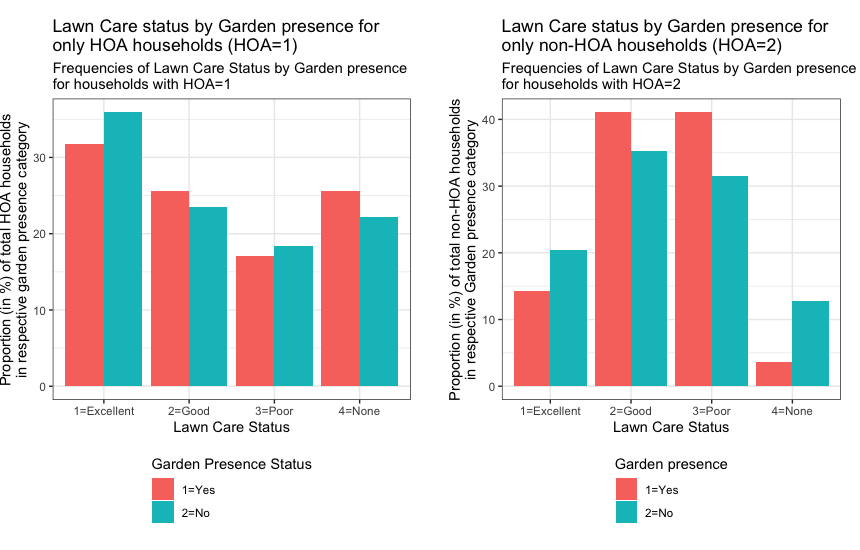
\includegraphics[scale=2]{LawnCareGarden.png}
\caption{Barplot for n=1616 households with 1059 households in HOA describing frequencies of \textbf{LawnCare status} by Garden presence of households as a percentage of total number of households in respective Garden presence category for a particular HOA category. \textbf{Left:} Only HOA households \textbf{Right:} Only non-HOA households} \label{Fig:Plot1}
\end{figure}

\textbf{Visual analysis}:

Looking at the contingency table and its visualization in Figure 6, we find no clear relationship between Lawn Care Status and Garden Presence Status for HOA households. The trend or distribution of proportion of HOA households within different Lawn Care statuses is same for both Garden Presence status (Yes, No). \\

The distribution of proportion of non-HOA households in different Lawn Care statuses is almost similar for households that have a garden and ones that don't too, except that there is an important discrepancy in this trend that must be noted. Within non-HOA households, we notice a relatively higher proportion of households who maintain None Lawn Care status for houses with a Garden than for the ones without a garden. In accordance with the evidence that we possess, no generalized relationship between Lawn Care and Garden presence may be concluded for non-HOA households. But it is important to note that there is a high tendency among non-HOA houses without a garden to have their lawns naturally managed than the houses which have a garden.\\

\textbf{Statistical tests}:

We will use the Chi-square independence hypothesis test to assess whether there is a statistically significant association between the variables Garden presence and Lawn Care Status. We shall be using this test separately for HOA and non-HOA households.

\textbf{HOA households}:

We first use the Chi-squared independence hypothesis test to test the following hypothesis for HOA households:\\

$H_{0}$: The Lawn Care status of HOA households is independent of the presence of a garden in these households

$H_{a}$: The Lawn Care status of HOA households is dependent on the presence of a garden in these households\\

\begin{Schunk}
\begin{Sinput}
> R1<-c(nrow(subset(dat.HOA, dat.HOA$HOA==1 & dat.HOA$Garden==1 
+     & dat.HOA$LawnCare==1)), 
+     nrow(subset(dat.HOA, dat.HOA$HOA==1 
+     & dat.HOA$Garden==1 & dat.HOA$LawnCare==2)), 
+     nrow(subset(dat.HOA, dat.HOA$HOA==1 & dat.HOA$Garden==1 
+     & dat.HOA$LawnCare==3)),
+     nrow(subset(dat.HOA, dat.HOA$HOA==1 & dat.HOA$Garden==1 & 
+     dat.HOA$LawnCare==4)))
> R2<-c(nrow(subset(dat.HOA, dat.HOA$HOA==1 & dat.HOA$Garden==2 
+     & dat.HOA$LawnCare==1)), 
+     nrow(subset(dat.HOA, dat.HOA$HOA==1 
+     & dat.HOA$Garden==2 & dat.HOA$LawnCare==2)), 
+     nrow(subset(dat.HOA, dat.HOA$HOA==1 & dat.HOA$Garden==2 
+     & dat.HOA$LawnCare==3)),
+     nrow(subset(dat.HOA, dat.HOA$HOA==1 & dat.HOA$Garden==2 & 
+     dat.HOA$LawnCare==4)))
> GardenLCH.tab<-matrix(data=c(R1,R2),
+                  nrow = 2,
+                  ncol = 4,
+                  byrow = TRUE)
> rownames(GardenLCH.tab)<-c("Yes","No")
> colnames(GardenLCH.tab)<-c("Excellent","Good", "Poor", "None")
> GardenLCH.tab
\end{Sinput}
\begin{Soutput}
    Excellent Good Poor None
Yes        26   21   14   21
No        351  229  180  217
\end{Soutput}
\end{Schunk}

Before proceeding with the test, we check the relevant assumptions.

1) The two variables are categorical.\\
- Garden presence: Yes, No\\
- Lawn Care status: Excellent, Good, Poor, None\\

2) The observations are independent\\
- It can be reasonably assumed that observations are independent- one observation's outcomes, whether in terms of HOA status or garden presence or any other variable of interest, doesn't affect later observations.\\
- Each sample can be represented in one and only one cell of the table.\\

3) The sample size is at least the number of cells in the table multiplied by 5;\\
- number of cells x 5= 8 x 5= 40 < 1059.\\

4) Expected count assumptions are met.

\begin{Schunk}
\begin{Sinput}
> ec_GardenLCH<-data.frame()
> for(i in 1:2){
+   counter<-c()
+   for(j in 1:4){
+     counter<-c(counter, (sum(GardenLCH.tab[i,])*sum(GardenLCH.tab[,j]))/1059)
+   }
+   ec_GardenLCH<-rbind(ec_GardenLCH, counter)
+ }
> rownames(ec_GardenLCH)<-c("Yes","No")
> colnames(ec_GardenLCH)<-c("Excellent","Good", "Poor", "None")
\end{Sinput}
\end{Schunk}

\begin{table}[H]
  \centering
    \begin{tabular}{|c|c|c|c|c|c|}\hline
    HOA &
    \backslashbox{Garden Presence}{Lawn Care Status} 
    & Excellent & Good & Poor & None \\\hline\hline
    
    Yes  & Yes &
    26 (29.19) & 21 (19.36) & 
    14 (15.02) & 
    21 (18.43)\\\hline\hline
    
    & No &
    351 (347.81) & 229 (230.64) & 
    180 (178.98) & 
    217 (219.57)\\\hline\hline
    
    \end{tabular}
    \caption{A contingency table for the Garden Presence and Lawn Care status of n=1616 observations categorized separately by HOA status (with expected count for each cell in parentheses)}
  \end{table}

100\% of the expected counts are greater than 5.

The assumptions are met, so we move forward with the test.

\begin{Schunk}
\begin{Sinput}
> chisq.test(GardenLCH.tab)
\end{Sinput}
\begin{Soutput}
	Pearson's Chi-squared test

data:  GardenLCH.tab
X-squared = 0.99345, df = 3, p-value = 0.8028
\end{Soutput}
\end{Schunk}

We obtain a p-value= 0.8028, which is greater than $\alpha$=0.05. Thus, we fail to reject the null hypothesis, that is, we fail to find evidence for statistically significant association between the variables Garden presence and Recycling status within HOA households. \\

\textbf{Non-HOA households}:

We now use the Chi-squared independence hypothesis test to test the following hypothesis for non-HOA households:\\

$H_{0}$: The Lawn Care status of non-HOA households is independent of the presence of a graden in these households

$H_{a}$: The Lawn Care status of non-HOA households is dependent on the presence of a garden in these households\\

\begin{Schunk}
\begin{Sinput}
> R1<-c(nrow(subset(dat.HOA, dat.HOA$HOA==2 & dat.HOA$Garden==1 
+     & dat.HOA$LawnCare==1)), 
+     nrow(subset(dat.HOA, dat.HOA$HOA==2 
+     & dat.HOA$Garden==1 & dat.HOA$LawnCare==2)), 
+     nrow(subset(dat.HOA, dat.HOA$HOA==2 & dat.HOA$Garden==1 
+     & dat.HOA$LawnCare==3)),
+     nrow(subset(dat.HOA, dat.HOA$HOA==2 & dat.HOA$Garden==1 & 
+     dat.HOA$LawnCare==4)))
> R2<-c(nrow(subset(dat.HOA, dat.HOA$HOA==2 & dat.HOA$Garden==2 
+     & dat.HOA$LawnCare==1)), 
+     nrow(subset(dat.HOA, dat.HOA$HOA==2 
+     & dat.HOA$Garden==2 & dat.HOA$LawnCare==2)), 
+     nrow(subset(dat.HOA, dat.HOA$HOA==2 & dat.HOA$Garden==2 
+     & dat.HOA$LawnCare==3)),
+     nrow(subset(dat.HOA, dat.HOA$HOA==2 & dat.HOA$Garden==2 & 
+     dat.HOA$LawnCare==4)))
> GardenLCNH.tab<-matrix(data=c(R1,R2),
+                  nrow = 2,
+                  ncol = 4,
+                  byrow = TRUE)
> rownames(GardenLCNH.tab)<-c("Yes","No")
> colnames(GardenLCNH.tab)<-c("Excellent","Good", "Poor", "None")
> GardenLCNH.tab
\end{Sinput}
\begin{Soutput}
    Excellent Good Poor None
Yes         8   23   23    2
No        102  177  158   64
\end{Soutput}
\end{Schunk}

Before proceeding with the test, we check the relevant assumptions.

1) The two variables are categorical.\\
- Garden presence: Yes, No\\
- Lawn Care status: Excellent, Good, Poor, None\\

2) The observations are independent\\
- It can be reasonably assumed that observations are independent- one observation's outcomes, whether in terms of HOA status or garden presence or any other variable of interest, doesn't affect later observations.\\
- Each sample can be represented in one and only one cell of the table.\\

3) The sample size is at least the number of cells in the table multiplied by 5;\\
- number of cells x 5= 8 x 5= 40 < 1059.\\

4) Expected count assumptions are met.

\begin{Schunk}
\begin{Sinput}
> ec_GardenLCNH<-data.frame()
> for(i in 1:2){
+   counter<-c()
+   for(j in 1:4){
+     counter<-c(counter, (sum(GardenLCNH.tab[i,])*sum(GardenLCNH.tab[,j]))/557)
+   }
+   ec_GardenLCNH<-rbind(ec_GardenLCNH, counter)
+ }
> rownames(ec_GardenLCNH)<-c("Yes","No")
> colnames(ec_GardenLCNH)<-c("Excellent","Good", "Poor", "None")
> ec_GardenLCNH
\end{Sinput}
\begin{Soutput}
    Excellent      Good      Poor      None
Yes  11.05925  20.10772  18.19749  6.635548
No   98.94075 179.89228 162.80251 59.364452
\end{Soutput}
\end{Schunk}

\begin{table}[H]
  \centering
    \begin{tabular}{|c|c|c|c|c|c|}\hline
    HOA &
    \backslashbox{Garden Presence}{Lawn Care Status} 
    & Excellent & Good & Poor & None \\\hline\hline
    
    No  & Yes &
    8 (11.06) & 23 (20.11) & 
    23 (18.2) & 
    2 (6.64)\\\hline\hline
    
    & No &
    102 (98.94) & 177 (179.89) & 
    158 (162.8) & 
    64 (59.36)\\\hline\hline
    
    \end{tabular}
    \caption{A contingency table for the Garden Presence and Lawn Care status of n=1616 observations categorized separately by HOA status (with expected counts for each cell in parantheses)}
  \end{table}

100\% of the expected counts are greater than 5.

The assumptions are met, so we move forward with the test.

\begin{Schunk}
\begin{Sinput}
> chisq.test(GardenLCNH.tab)
\end{Sinput}
\begin{Soutput}
	Pearson's Chi-squared test

data:  GardenLCNH.tab
X-squared = 6.4128, df = 3, p-value = 0.09317
\end{Soutput}
\end{Schunk}

We obtain a p-value= 0.09317, which is greater than $\alpha$=0.05. Thus, we fail to reject the null hypothesis, that is, we fail to find evidence for statistically significant association between the variables Garden presence and Recycling status within non-HOA households.

\textbf{Comparing the relationship across HOA status}: We fail to find evidence of a statistically significant relationship between the presence of a garden in a household and the sustainability of its lawn care status. Note that we find no association among the two variables of interest across both HOA status categories.

Overall, we conclude that the sustainability of lawn care status of a household is independent of the presence of a garden in it, regardless of its HOA status.

\section*{Relationship between Garden Presence and Recycling Status of households}

Table 15 below analyzes the frequencies of Recycling status by Garden presence separately for HOA and non-HOA households. 

\begin{Schunk}
\begin{Sinput}
> GR<-(prop.table(table(subset(dat.HOA, dat.HOA$HOA==1)$Garden,
+                                        subset(dat.HOA, dat.HOA$HOA==1)$Recycle),margin=1))*100
> GR2<-(prop.table(table(subset(dat.HOA, dat.HOA$HOA==2)$Garden,
+                                        subset(dat.HOA, dat.HOA$HOA==2)$Recycle),margin=1))*100
\end{Sinput}
\end{Schunk}

\begin{table}[H]
  \centering
    \begin{tabular}{|c|c|c|c|c|}\hline
    HOA &
    \backslashbox{Garden Presence}{Recycling Status}
    &$\begin{matrix} \text{1=Recycling bin}\\ \text{present} \end{matrix} $
    & $\begin{matrix} \text{2=Only trash bin}\\ \text{present} \end{matrix}$ 
    & $\begin{matrix} \text{3=Recycling bin status}\\ \text{unobservable under method}
    \\ \text{of data collection} \end{matrix}$ \\\hline\hline
    
    Yes  & Yes &
    58.54\% & 8.54\% & 
    32.93\%\\\hline\hline
    
    & No &
    57.93\% & 22.82\% & 
    19.24\% \\\hline\hline
    
    
    No  & Yes &
    73.21\% & 14.29\% & 
    12.5\% \\\hline\hline
    
    & No &
    66.27\% & 23.35\% & 
    10.38\% \\\hline\hline
    
    \end{tabular}
    \caption{A contingency table for the Garden Presence and Recycling status of n=1616 observations categorized separately by HOA status}
  \end{table}

We visualize the data in Table 15 in Figure 8.

\begin{Schunk}
\begin{Sinput}
> #create ggplot data frame
> library("cowplot") 
> tab_RecycleGarden<-(prop.table(table(subset(dat.HOA, dat.HOA$HOA==1)$Garden,
+                                        subset(dat.HOA, dat.HOA$HOA==1)$Recycle),margin=1))*100
> xlabs_RecycleGarden<-c("Recycle bin and\ntrash bin present",
+                        "Only trash bin\npresent", 
+                        "Unobservable (no curb side\npick-up)")
> ggdat<-data.frame(tab_RecycleGarden)
> p1<-ggplot(data=ggdat,aes(x=Var2,y=Freq,fill=as.factor(Var1)))+
+   geom_bar(stat="identity",
+            position="dodge")+
+   theme_bw()+
+   xlab("Recycling Status")+
+   ylab("Proportion (in %) of total HOA households\nin respective garden presence category")+
+   scale_fill_discrete(name="Garden Presence", labels= c("Yes","No"))+
+   ggtitle("Recycling status by Garden presence for\nonly HOA households (HOA=1)",
+           subtitle="Frequencies of Recycling Status by Garden presence\nfor 
+           households with HOA=1")+
+   scale_x_discrete(labels=xlabs_RecycleGarden)+
+   theme(legend.position = "bottom", legend.direction = "vertical")+
+   theme(plot.margin = unit(c(1, 1, 1, 0), "lines"))
> tab_RecycleGarden<-(prop.table(table(subset(dat.HOA, dat.HOA$HOA==2)$Garden,
+                                        subset(dat.HOA, dat.HOA$HOA==2)$Recycle),margin=1))*100
> xlabs_RecycleGarden<-c("Recycle bin and\ntrash bin present","Only trash bin\npresent",
+                        "Unobservable (no curb side\npick-up)")
> ggdat<-data.frame(tab_RecycleGarden)
> p2<-ggplot(data=ggdat,aes(x=Var2,y=Freq,fill=as.factor(Var1)))+
+   geom_bar(stat="identity",
+            position="dodge")+
+   theme_bw()+
+   xlab("Recycling Status")+
+   ylab("Proportion (in %) of total non-HOA households\nin respective Garden presence category")+
+   scale_fill_discrete(name="Garden presence", labels= c("Yes","No"))+
+   ggtitle("Recycling status by Garden presence for\nonly non-HOA households (HOA=2)", 
+           subtitle="Frequencies of Recycling Status by Garden presence\nfor households with
+           HOA=2")+
+   scale_x_discrete(labels=xlabs_RecycleGarden)+
+   theme(legend.position = "bottom", legend.direction = "vertical")+
+   theme(plot.margin = unit(c(1, 1, 1, 1), "lines"))
> grid.arrange(p1,p2,ncol=2)
\end{Sinput}
\end{Schunk}

\begin{figure}[H]
\centering
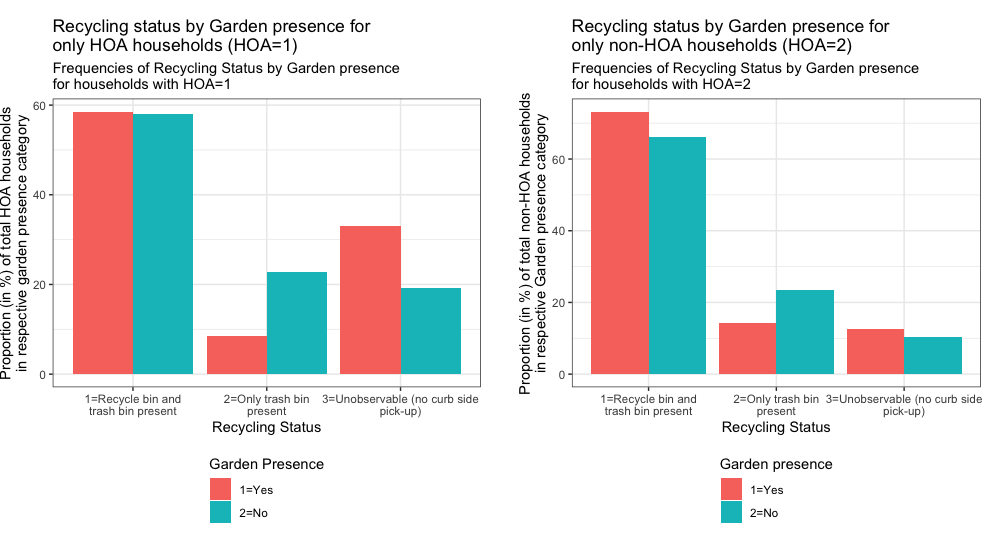
\includegraphics[scale=2]{RecycleGarden_final.png}
\caption{Barplot for n=1616 households with 1059 households in HOA describing frequencies of \textbf{Recycling status} by Garden presence of households as a percentage of total number of households in respective Garden presence category for a particular HOA category. \textbf{Left:} Only HOA households \textbf{Right:} Only non-HOA households} \label{Fig:Plot1}
\end{figure}

\textbf{Visual analysis}:

Within HOA households, the recycling tendency is almost similar among households that have a garden and the ones that do not. This is because the proportions of HOA households who recycle within 2 different categories of Garden presence is almost same. It also seems that households with a garden are more likely to be associated with neighborhoods with no curb side pickup, while households without a garden are more likely not to have a recycling bin present.\\

Within non-HOA households, households who have a garden have a slightly higher tendency to recycle, although I am not sure if this difference is statistically significant and suggests an associated between Garden presence and Recycling habits within non-HOA households.\\

\textbf{Statistical tests}:

We will use the Chi-square independence hypothesis test to assess whether there is a statistically significant association between the variables Garden presence and Recycling status. We shall be using this test separately for HOA and non-HOA households.

\textbf{HOA households}:

We first use the Chi-squared independence hypothesis test to test the following hypothesis for HOA households:\\

$H_{0}$: The Recycling status of HOA households is independent of the presence of a garden in these households

$H_{a}$: The Recycling status of HOA households is dependent on the presence of a garden in these households\\

\begin{Schunk}
\begin{Sinput}
> R1<-c(nrow(subset(dat.HOA, dat.HOA$HOA==1 & dat.HOA$Garden==1 
+     & dat.HOA$Recycle==1)), 
+     nrow(subset(dat.HOA, dat.HOA$HOA==1 
+     & dat.HOA$Garden==1 & dat.HOA$Recycle==2)), 
+     nrow(subset(dat.HOA, dat.HOA$HOA==1 & dat.HOA$Garden==1 
+     & dat.HOA$Recycle==3)))
> R2<-c(nrow(subset(dat.HOA, dat.HOA$HOA==1 & dat.HOA$Garden==2 
+     & dat.HOA$Recycle==1)), 
+     nrow(subset(dat.HOA, dat.HOA$HOA==1 
+     & dat.HOA$Garden==2 & dat.HOA$Recycle==2)), 
+     nrow(subset(dat.HOA, dat.HOA$HOA==1 & dat.HOA$Garden==2 
+     & dat.HOA$Recycle==3)))
> GardenRH.tab<-matrix(data=c(R1,R2),
+                  nrow = 2,
+                  ncol = 3,
+                  byrow = TRUE)
> rownames(GardenRH.tab)<-c("Yes","No")
> colnames(GardenRH.tab)<-c("Recycling bin","Only trash bin","Unobservable")
> GardenRH.tab
\end{Sinput}
\begin{Soutput}
    Recycling bin Only trash bin Unobservable
Yes            48              7           27
No            566            223          188
\end{Soutput}
\end{Schunk}

Before proceeding with the test, we check the relevant assumptions.

1) The two variables are categorical.\\
- Garden presence: Yes, No\\
- Recycling status: Both Recycling bin and trash bin present at the home, Only a trash bin was present, Recycling status unobservable under method of data collection (no curb-side pickup)\\

2) The observations are independent\\
- It can be reasonably assumed that observations are independent- one observation's outcomes, whether in terms of HOA status or garden presence or any other variable of interest, doesn't affect later observations.\\
- Each sample can be represented in one and only one cell of the table.\\

3) The sample size is at least the number of cells in the table multiplied by 5;\\
- number of cells x 5= 8 x 5= 40 < 1059.\\

4) Expected count assumptions are met.

\begin{Schunk}
\begin{Sinput}
> ec_GardenRH<-data.frame()
> for(i in 1:2){
+   counter<-c()
+   for(j in 1:3){
+     counter<-c(counter, (sum(GardenRH.tab[i,])*sum(GardenRH.tab[,j]))/1059)
+   }
+   ec_GardenRH<-rbind(ec_GardenRH, counter)
+ }
> rownames(ec_GardenRH)<-c("Yes","No")
> colnames(ec_GardenRH)<-c("Recycling bin","Only trash bin","Unobservable")
\end{Sinput}
\end{Schunk}

\begin{table}[H]
  \centering
    \begin{tabular}{|c|c|c|c|c|}\hline
    HOA &
    \backslashbox{Garden Presence}{Recycling Status}
    &$\begin{matrix} \text{1=Recycling bin}\\ \text{present} \end{matrix} $
    & $\begin{matrix} \text{2=Only trash bin}\\ \text{present} \end{matrix}$ 
    & $\begin{matrix} \text{3=Recycling bin status}\\ \text{unobservable under method}
    \\ \text{of data collection} \end{matrix}$ \\\hline\hline
    
    Yes  & Yes &
    48 (47.54) & 7 (17.81) & 
    27 (16.65)\\\hline\hline
    
    & No &
    566 (566.46) & 223 (212.19) & 
    188 (198.35) \\\hline\hline
    
    \end{tabular}
    \caption{A contingency table for the Garden Presence and Recycling status of n=1616 observations categorized separately by HOA status (with expected count for each cell in parantheses)}
  \end{table}

100\% of the expected counts are greater than 5.

The assumptions are met, so we move forward with the test.

\begin{Schunk}
\begin{Sinput}
> chisq.test(GardenRH.tab)
\end{Sinput}
\begin{Soutput}
	Pearson's Chi-squared test

data:  GardenRH.tab
X-squared = 14.094, df = 2, p-value = 0.0008701
\end{Soutput}
\end{Schunk}

We note a $p$-value of 0.0008701, which is less than $\alpha$=0.05. Thus, we have evidence to conclude that there is a statistically significant association between the variables Recycling status and garden presence within HOA households. We wish to use relevant statistical tests to verify if the nature of this association is as we noted in our visual analysis above.\\

\begin{Schunk}
\begin{Sinput}
> library(rcompanion)
> library(RVAideMemoire)
> # cramerV(GardenRH.tab, bias.correct=TRUE)
> cramer.test(GardenRH.tab, conf.level=0.95)
\end{Sinput}
\begin{Soutput}
	Cramér's association coefficient

data:  GardenRH.tab
X-squared = 14.094, df = 2, p-value = 0.0008701
alternative hypothesis: true association is not equal to 0
95 percent confidence interval:
 0.06516764 0.17357034
sample estimates:
        V 
0.1153626 
\end{Soutput}
\end{Schunk}

Since $k$= min(r,c)=min(2,3) =2, we note little to weak association between the two variables within HOA households.\\

In order to study the nature of the association between the two variables, we use the pairwise proportions test to assess the null hypothesis that there is no difference in any pair of proportions of households with and without a garden which fall within a particular Recycling Status category. Note that we apply the pairwise proportions test for each of the 3 Recycling status categories. Also note that we use the Benjamini-Hochberg method to cap the rate of Type I error at 5\%.

% Pairwise proportion tests

Having checked that the sample is representative of the population and that all observations are independent, we note that our sample fulfills the assumptions for the test.

\textbf{Both recycle and trash bin present}:

\begin{Schunk}
\begin{Sinput}
> pairwise.prop.test(x=c(GardenRH.tab["Yes","Recycling bin"],
+   GardenRH.tab["No", "Recycling bin"]), 
+       n=c(sum(GardenRH.tab["Yes",]), 
+       sum(GardenRH.tab["No",])),
+       p.adjust.method = "BH")
\end{Sinput}
\begin{Soutput}
	Pairwise comparisons using Pairwise comparison of proportions 

data:  c(GardenRH.tab["Yes", "Recycling bin"], GardenRH.tab["No", "Recycling bin"]) out of c(sum(GardenRH.tab["Yes", ]), sum(GardenRH.tab["No", ])) 

  1
2 1

P value adjustment method: BH 
\end{Soutput}
\end{Schunk}

We have no evidence to reject the null hypothesis ($p$-value>$\alpha$ for all pairs of proportions) and thus, we conclude that HOA households with and without a garden are equally likely to have a recycling bin present.

\textbf{Only trash bin present}:

\begin{Schunk}
\begin{Sinput}
> pairwise.prop.test(x=c(GardenRH.tab["Yes","Only trash bin"],
+   GardenRH.tab["No", "Only trash bin"]), 
+       n=c(sum(GardenRH.tab["Yes",]), 
+       sum(GardenRH.tab["No",])),
+       p.adjust.method = "BH")
\end{Sinput}
\begin{Soutput}
	Pairwise comparisons using Pairwise comparison of proportions 

data:  c(GardenRH.tab["Yes", "Only trash bin"], GardenRH.tab["No", "Only trash bin"]) out of c(sum(GardenRH.tab["Yes", ]), sum(GardenRH.tab["No", ])) 

  1    
2 0.004

P value adjustment method: BH 
\end{Soutput}
\end{Schunk}

Using the results of the pairwise proportion test and looking at the barplot in Figure 8, we have evidence to conclude that HOA households without a garden are more likely to have only a trash bin present, as compared to HOA households with a garden. This justifies visual evidence about the same we stated above.\\

\textbf{No curb side pickup}:

\begin{Schunk}
\begin{Sinput}
> pairwise.prop.test(x=c(GardenRH.tab["Yes","Unobservable"],
+   GardenRH.tab["No", "Unobservable"]), 
+       n=c(sum(GardenRH.tab["Yes",]), 
+       sum(GardenRH.tab["No",])),
+       p.adjust.method = "BH")
\end{Sinput}
\begin{Soutput}
	Pairwise comparisons using Pairwise comparison of proportions 

data:  c(GardenRH.tab["Yes", "Unobservable"], GardenRH.tab["No", "Unobservable"]) out of c(sum(GardenRH.tab["Yes", ]), sum(GardenRH.tab["No", ])) 

  1     
2 0.0049

P value adjustment method: BH 
\end{Soutput}
\end{Schunk}

Using the results of the pairwise proportion test and looking at the barplot in Figure 8, we have evidence to conclude that HOA households with a garden are more likely to have no curb side pickup, as compared to HOA households without a garden. This also justifies the visual evidence that we stated above.\\

\textbf{Non-HOA households}:

We now use the Chi-squared independence hypothesis test to test the following hypothesis for non-HOA households:\\

$H_{0}$: The Recycling status of non-HOA households is independent of the presence of a garden in these households

$H_{a}$: The Recycling status of non-HOA households is dependent on the presence of a garden in these households\\

\begin{Schunk}
\begin{Sinput}
> R1<-c(nrow(subset(dat.HOA, dat.HOA$HOA==2 & dat.HOA$Garden==1 
+     & dat.HOA$Recycle==1)), 
+     nrow(subset(dat.HOA, dat.HOA$HOA==2 
+     & dat.HOA$Garden==1 & dat.HOA$Recycle==2)), 
+     nrow(subset(dat.HOA, dat.HOA$HOA==2 & dat.HOA$Garden==1 
+     & dat.HOA$Recycle==3)))
> R2<-c(nrow(subset(dat.HOA, dat.HOA$HOA==2 & dat.HOA$Garden==2 
+     & dat.HOA$Recycle==1)), 
+     nrow(subset(dat.HOA, dat.HOA$HOA==2 
+     & dat.HOA$Garden==2 & dat.HOA$Recycle==2)), 
+     nrow(subset(dat.HOA, dat.HOA$HOA==2 & dat.HOA$Garden==2 
+     & dat.HOA$Recycle==3)))
> GardenRNH.tab<-matrix(data=c(R1,R2),
+                  nrow = 2,
+                  ncol = 3,
+                  byrow = TRUE)
> rownames(GardenRNH.tab)<-c("Yes","No")
> colnames(GardenRNH.tab)<-c("Recycling bin","Only trash bin","Unobservable")
> GardenRNH.tab
\end{Sinput}
\begin{Soutput}
    Recycling bin Only trash bin Unobservable
Yes            41              8            7
No            332            117           52
\end{Soutput}
\end{Schunk}

Before proceeding with the test, we check the relevant assumptions.

1) The two variables are categorical.\\
- Garden presence: Yes, No\\
- Recycling status: Both Recycling bin and trash bin present at the home, Only a trash bin was present, Recycling status unobservable under method of data collection (no curb-side pickup)\\

2) The observations are independent\\
- It can be reasonably assumed that observations are independent- one observation's outcomes, whether in terms of HOA status or garden presence or any other variable of interest, doesn't affect later observations.\\
- Each sample can be represented in one and only one cell of the table.\\

3) The sample size is at least the number of cells in the table multiplied by 5;\\
- number of cells x 5= 8 x 5= 40 < 1059.\\

4) Expected count assumptions are met.

\begin{Schunk}
\begin{Sinput}
> ec_GardenRNH<-data.frame()
> for(i in 1:2){
+   counter<-c()
+   for(j in 1:3){
+     counter<-c(counter, (sum(GardenRNH.tab[i,])*sum(GardenRNH.tab[,j]))/1059)
+   }
+   ec_GardenRNH<-rbind(ec_GardenRNH, counter)
+ }
> rownames(ec_GardenRNH)<-c("Yes","No")
> colnames(ec_GardenRNH)<-c("Recycling bin","Only trash bin","Unobservable")
\end{Sinput}
\end{Schunk}

\begin{table}[H]
  \centering
    \begin{tabular}{|c|c|c|c|c|}\hline
    HOA &
    \backslashbox{Garden Presence}{Recycling Status}
    &$\begin{matrix} \text{1=Recycling bin}\\ \text{present} \end{matrix} $
    & $\begin{matrix} \text{2=Only trash bin}\\ \text{present} \end{matrix}$ 
    & $\begin{matrix} \text{3=Recycling bin status}\\ \text{unobservable under method}
    \\ \text{of data collection} \end{matrix}$ \\\hline\hline
    
    No  & Yes &
    41 (19.72) & 8 (6.61) & 
    7 (3.12) \\\hline\hline
    
    & No &
    332 (176.46) & 117 (59.14) & 
    52 (27.91) \\\hline\hline
    
    \end{tabular}
    \caption{A contingency table for the Garden Presence and Recycling status of n=1616 observations categorized separately by HOA status (with expected counts for each cell in parantheses)}
  \end{table}


100\% of the expected counts are greater than 5.

The assumptions are met, so we move forward with the test.

\begin{Schunk}
\begin{Sinput}
> chisq.test(GardenRNH.tab)
\end{Sinput}
\begin{Soutput}
	Pearson's Chi-squared test

data:  GardenRNH.tab
X-squared = 2.4223, df = 2, p-value = 0.2979
\end{Soutput}
\end{Schunk}

We note a $p$-value of 0.2979, which is greater than $\alpha$=0.05. We fail to reject the null hypothesis and conclude that there is no statistically significant association between the variables Recycling status and Garden presence within non-HOA households.

\textbf{Summarizing analysis}: We note no statistiaclly significant association between Recycling status and garden presence within non-HOA households. Thus, we note that the presence of garden is unlikely to determine the recycling habits of a household which is not a member of homeowners' association.\\

Within HOA households, though, it is interesting to note that both households with and without a garden are equally likely to have a recycling bin present. However, HOA households with a garden are relatively less likely to have curb side pickup. This may also be the reason that HOA households with a garden are relatively less likely to have a trash bin present.\\

\section*{Relationship between Tree Planting tendency and Lawn Care Status of households}

Table 18 shows the numerical summary of number of trees planted within different Lawn Care statuses across both HOA status categories. We visualize this data in Figure 9.

\begin{Schunk}
\begin{Sinput}
> hoaT<-tapply(X=subset(dat.HOAn, dat.HOAn$HOA==1)$Trees,
+     INDEX = subset(dat.HOAn, dat.HOAn$HOA==1)$ LawnCare, summary)
> nonhoaT<- tapply(X=subset(dat.HOAn, dat.HOAn$HOA==2)$Trees,
+     INDEX = subset(dat.HOAn, dat.HOAn$HOA==2)$LawnCare, summary)
\end{Sinput}
\end{Schunk}

\begin{table}[H]
  \centering
    \begin{tabular}{|c|c|c|c|c|c|c|c|}\hline
    HOA &
    Lawn Care Status 
    & Min. & 1st Qu. & Median & Mean & 3rd Qu. & Max. \\\hline\hline
    
    Yes & Excellent &
    0 & 1 & 
    2 & 
    2.739 & 4 & 18\\\hline\hline
    
    & Good &
    0 & 1 & 
    2.5 & 
    3.032 & 4 & 18\\\hline\hline
    
    & Poor &
    0 & 1 & 
    2 & 
    3.077 & 4 & 22 \\\hline\hline
    
    & None &
    0 & 1 & 
    2 & 
    3.081 & 4 & 35\\\hline\hline
    
   No & Excellent &
    0 & 2.75 & 
    5 & 
    5.889 & 9 & 28\\\hline\hline
    
    & Good &
    0 & 3 & 
    5 & 
    6.467 & 8 & 40\\\hline\hline
    
    & Poor &
    0 & 2 & 
    4 & 
    5.017 & 7 & 25 \\\hline\hline
    
    & None &
    0 & 3 & 
    6.5 & 
    6.633 & 10 & 15\\\hline\hline
    
    \end{tabular}
    \caption{Numerical summary of number of trees planted across different Lawn Care statuses within each HOA category}
  \end{table}

\begin{Schunk}
\begin{Sinput}
> library("ggplot2") 
> library("gridExtra")
> xlabsLC<-c("Excellent", "Good", "Poor", "None")
> p1<-ggplot(subset(dat.HOAn, dat.HOAn$HOA==1), aes(x=as.factor(LawnCare), y=Trees)) + 
+   geom_violin(fill="lightblue",    
+               trim = FALSE,
+               alpha = 0.9, 
+               show.legend = FALSE,
+               position=position_dodge(width=0.9))+
+   geom_boxplot(width = 0.15, fill="white", position=position_dodge(width=0.9))+
+   #plot smaller boxplot inside violin
+   xlab("Lawn Care Status")+ #x axis label
+   ylab("Number of Trees")    + #y axis label
+   ggtitle("Number of Trees in the front yard", subtitle = "Includes 1056 HOA households") + #add title to plot
+   theme_bw()+  #removes grey background
+   scale_x_discrete(labels=xlabsLC)
> p2<-ggplot(subset(dat.HOAn, dat.HOAn$HOA==2), aes(x=as.factor(LawnCare), y=Trees)) + 
+   geom_violin(fill="lightblue",    
+               trim = FALSE,
+               alpha = 0.9, 
+               show.legend = FALSE,
+               position=position_dodge(width=0.9))+
+   geom_boxplot(width = 0.15, fill="white", position=position_dodge(width=0.9))+
+   #plot smaller boxplot inside violin
+   xlab("Lawn Care Status")+ #x axis label
+   ylab("Number of Trees")    + #y axis label
+   ggtitle("Number of Trees in the front yard", subtitle = "Includes 546 non-HOA households") + #add title to plot
+   theme_bw()+  #removes grey background
+   scale_x_discrete(labels=xlabsLC)
> grid.arrange(p1,p2,ncol=2)
\end{Sinput}
\end{Schunk}

\begin{figure}[H]
\centering
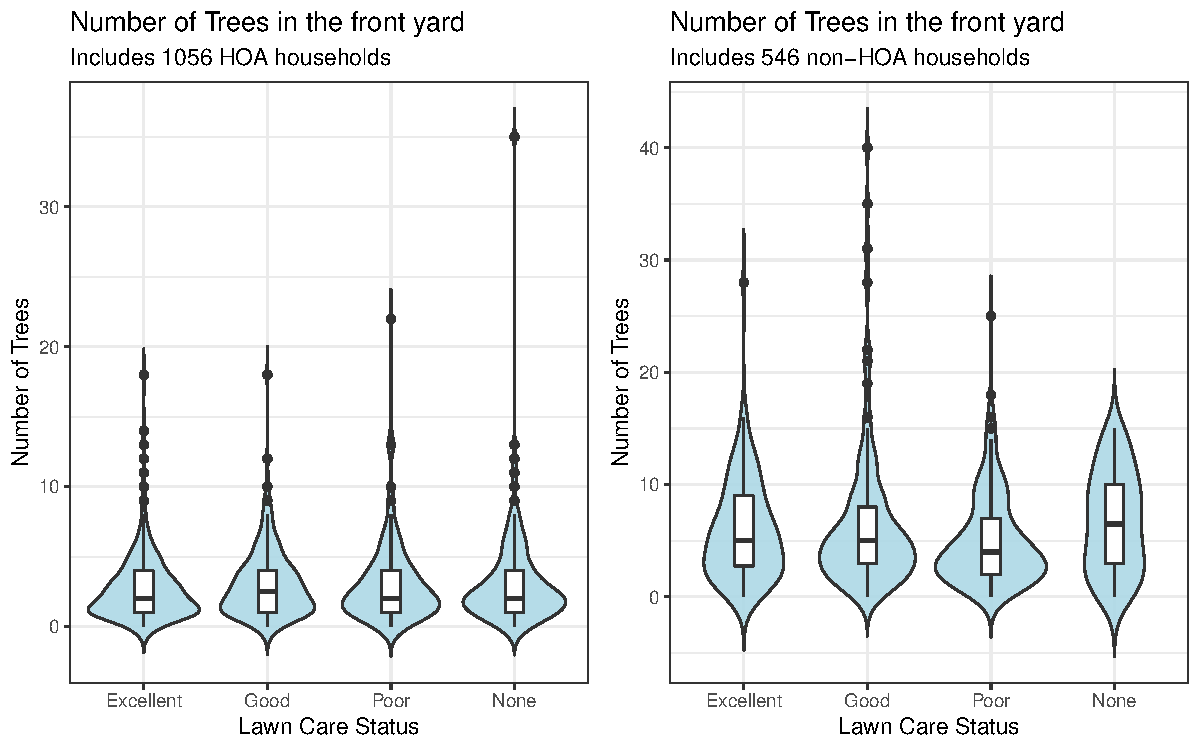
\includegraphics{part2-074}
\caption{Violin plot (with embedded boxplot) visualizing the distribution of number of trees across households with different Lawn Care statuses which are \textbf{Right:} members of HOA \textbf{Left}: not members of HOA} \label{Fig:plot1}
\end{figure}

\textbf{Visual analysis}:

We firstly note that the data on number of trees is highly right skewed across all Lawn Care status categories, regardless of HOA status. Thus, we note that the median number of trees must be used to compare tree planting tendencies among households maintaining different Lawn Care statuses in a particular HOA status category. \\

Within HOA households, we do not note any noticeable differences in the median number of trees planted by households maintaining different Lawn Care statuses. Within non-HOA households, however, we believe that a household having their lawn be fully artificially managed is more likely to have a higher number of trees relative to a a household maintaining any other Lawn Care status.\\

\textbf{Statistical tests}:

We can apply the Mood's Median test to check if there are any statistically significant differences among the median number of trees planted by households with a particular HOA status which maintain different Lawn Care statuses. Note that we apply this test separately for HOA and non-HOA households.

\textbf{HOA households}:

We test the following hypotheses:

$H_{0}$: $M_{1}=M_{2}=M_{3}=M_{4}$

$H_{a}$: The population medians $M_{i}$ are not all equal\\

where, $M_{1}$: the median number of trees planted by HOA households maintaining Excellent Lawn Care status

$M_{2}$: the median number of trees planted by HOA households maintaining Good Lawn Care status

$M_{3}$: the median number of trees planted by HOA households maintaining Poor Lawn Care status

$M_{4}$: the median number of trees planted by HOA households maintaining None Lawn Care status\\

We first check that the available sample data satisfies the necessary assumptions for the Mood's Median test:

1) The sample is generalizable to the population of interest. We assume that the researcher's methodology for collecting data for the study did not introduce any bias. Thus, our samples are generalizable to their respective population HOA and non-HOA households.\\

2) The observations are independent, as no observation affects other observed data. The samples are thus representative of their respective populations.\\

Having checked the assumptions, we proceed with the test.

\begin{Schunk}
\begin{Sinput}
> mood.medtest(Trees~LawnCare, 
+           data=subset(dat.HOAn, dat.HOAn$HOA==1)) # not significant
\end{Sinput}
\begin{Soutput}
	Mood's median test

data:  Trees by LawnCare
X-squared = 2.7752, df = 3, p-value = 0.4276
\end{Soutput}
\end{Schunk}

As we predicted in our visual analysis, we fail to find any statistically significant differences in the median number of trees planted by HOA households across different Lawn Care statuses.\\

\textbf{Non-HOA households}:

We note that both assumptions also hold for non-HOA households, and we proceed with the test.

\begin{Schunk}
\begin{Sinput}
> mood.medtest(Trees~LawnCare, 
+           data=subset(dat.HOAn, dat.HOAn$HOA==2))
\end{Sinput}
\begin{Soutput}
	Mood's median test

data:  Trees by LawnCare
X-squared = 10.897, df = 3, p-value = 0.01229
\end{Soutput}
\end{Schunk}

We obtain a $p$-value< $\alpha$=0.05. We thus reject the null hypothesis and conduct a post hoc test to specifically understand which medians are different, and the nature of difference.

\textbf{Post-Hoc testing}:

\begin{Schunk}
\begin{Sinput}
> library(rcompanion)
> garbage<-invisible(capture.output(PT<-pairwiseMedianTest(Trees~LawnCare,
+     data= subset(dat.HOAn, dat.HOAn$HOA==2), method= "BH")))
> cldList(p.adjust ~ Comparison,
+         data = PT,
+         threshold = 0.05)
\end{Sinput}
\begin{Soutput}
  Group Letter MonoLetter
1     1     ab         ab
2     2     ab         ab
3     3      a         a 
4     4      b          b
\end{Soutput}
\end{Schunk}

\textbf{Note:} For Lawn Care status: 1= Excellent, 2= Good, 3= Poor and 4= None.\\

Within non-HOA households, we note a statistically significant difference between the median number of trees planted by households which maintain Poor Lawn Care status relative to houses which maintain None Lawn Care status. In our visual analysis, we predicted that the median number of trees planted by households with lawns fully artificially managed would be higher relative to the median number of trees planted by households maintaining any other Lawn Care status. However, we obtain such a result only for the households maintaining Poor and None Lawn Care status.\\

Overall, however, we do not find evidence that the Lawn Care status is a good predictor for number of trees, even for non-HOA households. \\

\textbf{Summarizing analysis}: In accordance with the statistical analysis which supports our visual insight, we note that no significant association exists between the variables Lawn Care Status and number of trees planted, regardless of HOA status.

\section*{Relationship between Tree Planting tendency and Garden presence of households}

Table 19 shows the numerical summary of number of trees planted within different Garden presence categories across both HOA status categories. We visualize this data in Figure 10.

\begin{Schunk}
\begin{Sinput}
> hoaG<-tapply(X=subset(dat.HOAn, dat.HOAn$HOA==1)$Trees,
+     INDEX = subset(dat.HOAn, dat.HOAn$HOA==1)$ Garden, summary)
> nonhoaG<- tapply(X=subset(dat.HOAn, dat.HOAn$HOA==2)$Trees,
+     INDEX = subset(dat.HOAn, dat.HOAn$HOA==2)$Garden, summary)
\end{Sinput}
\end{Schunk}

\begin{table}[H]
  \centering
    \begin{tabular}{|c|c|c|c|c|c|c|c|}\hline
    HOA &
    Garden Presence
    & Min. & 1st Qu. & Median & Mean & 3rd Qu. & Max. \\\hline\hline
    
    Yes & Yes &
    0 & 1 & 
    2.5 & 
    2.988 & 4 & 10\\\hline\hline
    
    & No &
    0 & 1 & 
    2 & 
    2.944 & 4 & 35\\\hline\hline
    
   No & Yes &
    1 & 2 & 
    4 & 
    4.554 & 6 & 15\\\hline\hline
    
    & No &
    0 & 2 & 
    5 & 
    6.049 & 9 & 40\\\hline\hline
    
    \end{tabular}
    \caption{Numerical summary of number of trees planted across different Garden presence categories within each HOA category}
  \end{table}

\begin{Schunk}
\begin{Sinput}
> library("ggplot2") 
> library("gridExtra")
> xlabsG<-c("Yes", "No")
> p1<-ggplot(subset(dat.HOAn, dat.HOAn$HOA==1), aes(x=as.factor(Garden), y=Trees)) + 
+   geom_violin(fill="lightblue",    
+               trim = FALSE,
+               alpha = 0.9, 
+               show.legend = FALSE,
+               position=position_dodge(width=0.9))+
+   geom_boxplot(width = 0.15, fill="white", position=position_dodge(width=0.9))+
+   #plot smaller boxplot inside violin
+   xlab("Garden presence")+ #x axis label
+   ylab("Number of Trees")    + #y axis label
+   ggtitle("Number of Trees in the front yard", subtitle = "Includes 1056 HOA households") + #add title to plot
+   theme_bw()+  #removes grey background
+   scale_x_discrete(labels=xlabsG)
> p2<-ggplot(subset(dat.HOAn, dat.HOAn$HOA==2), aes(x=as.factor(Garden), y=Trees)) + 
+   geom_violin(fill="lightblue",    
+               trim = FALSE,
+               alpha = 0.9, 
+               show.legend = FALSE,
+               position=position_dodge(width=0.9))+
+   geom_boxplot(width = 0.15, fill="white", position=position_dodge(width=0.9))+
+   #plot smaller boxplot inside violin
+   xlab("Garden presence")+ #x axis label
+   ylab("Number of Trees")    + #y axis label
+   ggtitle("Number of Trees in the front yard", subtitle = "Includes 556 non-HOA households") + #add title to plot
+   theme_bw()+  #removes grey background
+   scale_x_discrete(labels=xlabsG)
> grid.arrange(p1,p2,ncol=2)
\end{Sinput}
\end{Schunk}

\begin{figure}[H]
\centering
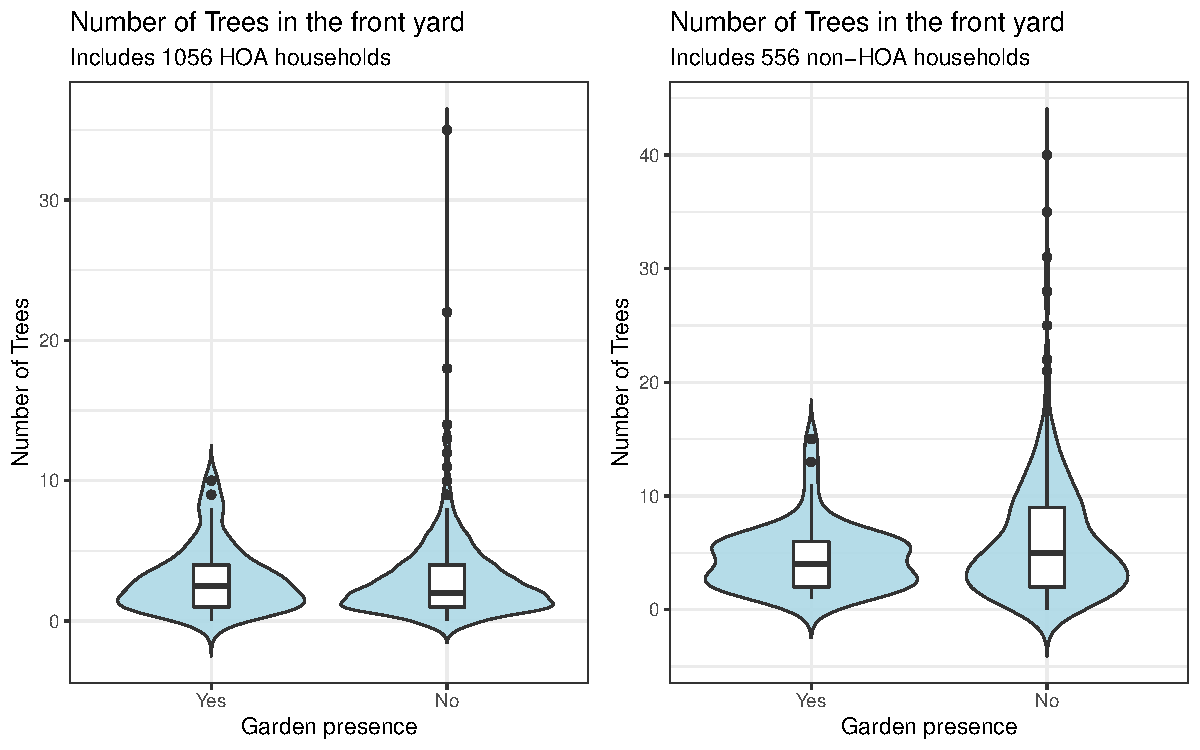
\includegraphics{part2-080}
\caption{Violin plot (with embedded boxplot) visualizing the distribution of number of trees across households with different garden presence categories which are \textbf{Right:} members of HOA \textbf{Left}: not members of HOA} \label{Fig:plot1}
\end{figure}

\textbf{Visual analysis}:

We firstly note that the data on number of trees is highly right skewed across households with and without a garden, regardless of HOA status. Thus, we note that the median number of trees must be used to compare tree planting tendencies among households maintaining different Lawn Care statuses in a particular HOA status category. \\

We do not notice any significant differences in medians between households with and without a garden, regardless of HOA status of households. It seems that there is no noticeable or clear relationship between the number of trees planted by a households and the presence of a garden in it, regardless of the HOA status of the household.\\

\textbf{Statistical tests}:

We can apply the Mood's Median test to check if there are any statistically significant differences among the median number of trees planted by households with a particular HOA status which either have or don't have a garden. Note that we apply this test separately for HOA and non-HOA households.

\textbf{HOA households}:

We test the following hypotheses:

$H_{0}$: $M_{1}=M_{2}$

$H_{a}$: $M_{1} \neq M_{2}$\\

where, $M_{1}$: the median number of trees planted by HOA households which have a garden present

$M_{2}$: the median number of trees planted by HOA households which don't have a garden present\\

We first check that the available sample data satisfies the necessary assumptions for the Mood's Median test:

1) The sample is generalizable to the population of interest. We assume that the researcher's methodology for collecting data for the study did not introduce any bias. Thus, our samples are generalizable to their respective population HOA and non-HOA households.\\

2) The observations are independent, as no observation affects other observed data. The samples are thus representative of their respective populations.\\

Having checked the assumptions, we proceed with the test.

\begin{Schunk}
\begin{Sinput}
> mood.medtest(Trees~Garden, 
+           data=subset(dat.HOAn, dat.HOAn$HOA==1))
\end{Sinput}
\begin{Soutput}
	Mood's median test

data:  Trees by Garden
X-squared = 0.50291, df = 1, p-value = 0.4782
\end{Soutput}
\end{Schunk}

As we predicted in our visual analysis, we fail to find any statistically significant differences in the median number of trees planted by HOA households across different garden presence categories.\\

\textbf{Non-HOA households}:

We note that both assumptions also hold for non-HOA households, and we proceed with the test.

\begin{Schunk}
\begin{Sinput}
> mood.medtest(Trees~Garden, 
+           data=subset(dat.HOAn, dat.HOAn$HOA==2))
\end{Sinput}
\begin{Soutput}
	Mood's median test

data:  Trees by Garden
X-squared = 0.50352, df = 1, p-value = 0.478
\end{Soutput}
\end{Schunk}

As we predicted in our visual analysis, we fail to find any statistically significant differences in the median number of trees planted by non-HOA households across different garden presence categories.\\

\textbf{Summarizing analysis}: We conclude that no statistically significant relationship exists between the presence of a garden in a house and the number of trees planted. In other words, the presence of a garden in a house is unlikely to predict the number of trees planted.\\

\section*{Relationship between Tree Planting tendency and Recycling of households}

Table 20 shows the numerical summary of number of trees planted within different Recycling status categories across both HOA status categories. We visualize this data in Figure 11.

\begin{Schunk}
\begin{Sinput}
> hoaR<-tapply(X=subset(dat.HOAn, dat.HOAn$HOA==1)$Trees,
+     INDEX = subset(dat.HOAn, dat.HOAn$HOA==1)$ Recycle, summary)
> nonhoaR<- tapply(X=subset(dat.HOAn, dat.HOAn$HOA==2)$Trees,
+     INDEX = subset(dat.HOAn, dat.HOAn$HOA==2)$Recycle, summary)
\end{Sinput}
\end{Schunk}

\begin{table}[H]
  \centering
    \begin{tabular}{|c|c|c|c|c|c|c|c|}\hline
    HOA &
    Garden Presence
    & Min. & 1st Qu. & Median & Mean & 3rd Qu. & Max. \\\hline\hline
    
    Yes & Recycling bin present &
    0 & 1 & 
    3 & 
    3.278 & 4 & 35\\\hline\hline
    
    & Only trash bin present &
    0 & 1 & 
    2 & 
    2.764 & 4 & 13\\\hline\hline
    
    & Unobservable Recycling status &
    0 & 1 & 
    1 & 
    2.2 & 3 & 14\\\hline\hline
    
   No & Recycling bin present &
    0 & 3 & 
    5 & 
    6.099 & 8 & 40\\\hline\hline
    
    & Only trash bin present &
    1 & 3 & 
    5 & 
    6.145 & 9 & 28\\\hline\hline
    
    & Unobservable Recycling status &
    0 & 1 & 
    2 & 
    4.119 & 6 & 16\\\hline\hline
    
    \end{tabular}
    \caption{Numerical summary of number of trees planted across different Recycling status categories within each HOA category}
  \end{table}

\begin{Schunk}
\begin{Sinput}
> library("ggplot2") 
> library("gridExtra")
> xlabsR<-c("Recycling bin present", "Only trash bin", "No curb side\npickup")
> p1<-ggplot(subset(dat.HOAn, dat.HOAn$HOA==1), aes(x=as.factor(Recycle), y=Trees)) + 
+   geom_violin(fill="lightblue",    
+               trim = FALSE,
+               alpha = 0.9, 
+               show.legend = FALSE,
+               position=position_dodge(width=0.9))+
+   geom_boxplot(width = 0.15, fill="white", position=position_dodge(width=0.9))+
+   #plot smaller boxplot inside violin
+   xlab("Recycling status")+ #x axis label
+   ylab("Number of Trees")    + #y axis label
+   ggtitle("Number of Trees in the front yard", subtitle = "Includes 1056 HOA households") + #add title to plot
+   theme_bw()+  #removes grey background
+   scale_x_discrete(labels=xlabsR)
> p2<-ggplot(subset(dat.HOAn, dat.HOAn$HOA==2), aes(x=as.factor(Recycle), y=Trees)) + 
+   geom_violin(fill="lightblue",    
+               trim = FALSE,
+               alpha = 0.9, 
+               show.legend = FALSE,
+               position=position_dodge(width=0.9))+
+   geom_boxplot(width = 0.15, fill="white", position=position_dodge(width=0.9))+
+   #plot smaller boxplot inside violin
+   xlab("Recycling status")+ #x axis label
+   ylab("Number of Trees")    + #y axis label
+   ggtitle("Number of Trees in the front yard", subtitle = "Includes 556 non-HOA households") + #add title to plot
+   theme_bw()+  #removes grey background
+   scale_x_discrete(labels=xlabsR)
> grid.arrange(p1,p2,ncol=2)
\end{Sinput}
\end{Schunk}

\begin{figure}[H]
\centering
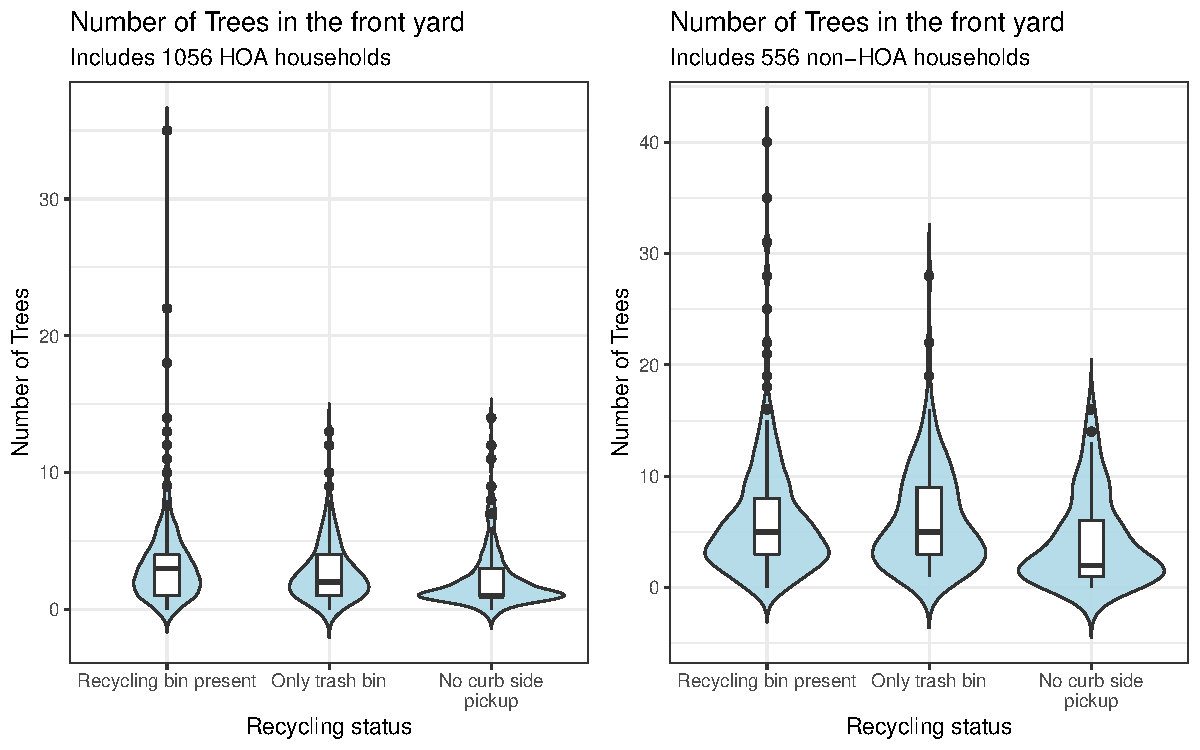
\includegraphics{part2-085}
\caption{Violin plot (with embedded boxplot) visualizing the distribution of number of trees across households with different recycling status categories which are \textbf{Right:} members of HOA \textbf{Left}: not members of HOA} \label{Fig:plot1}
\end{figure}

\textbf{Visual analysis}:

We firstly note that the data on number of trees is highly right skewed across all Recycling status categories, regardless of HOA status. Thus, we note that the median number of trees must be used to compare tree planting tendencies among households maintaining different Lawn Care statuses in a particular HOA status category. \\

Within HOA households, we see a noticeable relationship between the two variables of interest. It seems that HOA households with a recycling bin are more likely to have a higher number of trees relative to HOA houses with only a trash bin and those with no curb side pikcup.\\

Within non-HOA households, however, we do not find any clear association between recycling habits and tree planting tendencies of households.\\

\textbf{Statistical tests}:

We can apply the Mood's Median test to check if there are any statistically significant differences among the median number of trees planted by households with a particular HOA status which either have or don't have a garden. Note that we apply this test separately for HOA and non-HOA households.

\textbf{HOA households}:

We test the following hypotheses:

$H_{0}$: $M_{1}=M_{2}=M_{3}$

$H_{a}$: the population median $M_{i}$ are not all equal\\

where, $M_{1}$: the median number of trees planted by HOA households which have a recycling bin present

$M_{2}$: the median number of trees planted by HOA households which only have a trash bin present

$M_{3}$: the median number of trees planted by HOA households with unobservable recycling status\\

We first check that the available sample data satisfies the necessary assumptions for the Mood's Median test:

1) The sample is generalizable to the population of interest. We assume that the researcher's methodology for collecting data for the study did not introduce any bias. Thus, our samples are generalizable to their respective population HOA and non-HOA households.\\

2) The observations are independent, as no observation affects other observed data. The samples are thus representative of their respective populations.\\

Having checked the assumptions, we proceed with the test.

\begin{Schunk}
\begin{Sinput}
> mood.medtest(Trees~Recycle, 
+           data=subset(dat.HOAn, dat.HOAn$HOA==1))
\end{Sinput}
\begin{Soutput}
	Mood's median test

data:  Trees by Recycle
X-squared = 49.625, df = 2, p-value = 1.676e-11
\end{Soutput}
\end{Schunk}

We note that the $p$-value is less than $\alpha$=0.05, which means we have evidence to reject the null hypothesis. We conduct post-hoc testing to further explore which particular medians are different, and the nature of this (these) difference(s).

\textbf{Post-Hoc testing}:

\begin{Schunk}
\begin{Sinput}
> library(rcompanion)
> garbage<-invisible(capture.output(PT<-pairwiseMedianTest(Trees~Recycle,
+     data= subset(dat.HOAn, dat.HOAn$HOA==1), method= "BH")))
> cldList(p.adjust ~ Comparison,
+         data = PT,
+         threshold = 0.05)
\end{Sinput}
\begin{Soutput}
  Group Letter MonoLetter
1     1      a        a  
2     2      b         b 
3     3      c          c
\end{Soutput}
\end{Schunk}

\textbf{Note:} For Recycling status: 1= Recycling bin present, 2= Only trash bin present, 3= Unobservable recycling status.\\

Within HOA households, we find evidence that the median number of trees planted by households is statistically different among houses with different recycling statuses. Using our visual insight and the results of the pairwise post-hoc test, it is clear that HOA households with a recycling bin are most likely to have the highest number of trees planted relative to houses with the other two recycling statuses. Furthermore, the number of trees planted by HOA households without a trash bin are likely to be more relative to households without curb side pickup. \\

Here, we find association between the variables Trees planted by a house and its recycling status. \textbf{More sustainable recycling habits leads to more sustainable tree planting tendencies, which is an important result from a policy standpoint}.\\

\textbf{Non-HOA households}:

We note that both assumptions also hold for non-HOA households, and we proceed with the test.

\begin{Schunk}
\begin{Sinput}
> mood.medtest(Trees~Recycle, 
+           data=subset(dat.HOAn, dat.HOAn$HOA==2))
\end{Sinput}
\begin{Soutput}
	Mood's median test

data:  Trees by Recycle
X-squared = 5.3359, df = 2, p-value = 0.06939
\end{Soutput}
\end{Schunk}

We note that the $p$-value=0.06939 is greater than $\alpha$=0.05. We fail to find any statistically significant differences in median number of trees planted by non-HOA households across different HOA statuses.\\

\textbf{Summarizing analysis}: We find an association between Trees planted and recycling status within HOA households, where more sustainable recycling tendency is associated with more sustainable tree planting habits.\\

\section*{Relationship among multiple sustainability indicators: An overall assessment}

Overall, two results are of interest in answering our research question. Within HOA households, we find that sustainable recycling tendency is weakly associated with extremely unsustainable lawn care status and sustainable tree planting tendencies. We fail to find any statistically significant association among two variables of interest within non-HOA households. \\

This may imply that the norms and regulations governing households that are a part of homeowners' association may impact the sustainability of these households in two ways. First, they have an impact on their tree planting, recycling and lawn care maintenance tendencies relative to those of non-HOA households. Secondly, they have an indirect impact. They lead to weak associations among multiple sustainability criteria within HOA households, while no such associations are seen in case of non-HOA households. Understanding the reasons for the existence of such relationships among HOA households may help us gain better insight into the specific policies and regulations of HOA that influence sustainability at the homeowner level.\\

\section*{Author's conclusion}

We conclude by saying that non-HOA households show relatively better sustainability habits, in terms of individual sustainability indicators at the homeowner level. Specifically, the median number of trees planted by HOA households is relatively higher and non-HOA households are relatively more likely to have a recycling bin present. We note only a weak association among the variables HOA status and trees planted, HOA status and recycling status and HOA status and Lawn Care status of households. Even with the weak association, however, we note clear insights into the differences in sustainability habits, at the homeowner level, across HOA status.\\

We also note that being a member of a homewoners' association has a major impact on the relationship among multiple sustainability indicators within HOA households. We noted that HOA households' sustainable recycling tendency is linked to extremely unsustainable lawn care status and sustainable tree planting tendencies. This not only has important policy implications, but also may offer insight into the impact of HOA status in influencing sustainablity outcomes of a households.\\

Overall, we see this analysis as a valuable contribution to better inform the researcher and the existing literature on how sustaibility outcomes, measured in terms of individual sustainability indicators, as well as relationship between multiple sustainability indicators vary across HOA statuses.\\

\section*{Topics for further research}

\begin{itemize}

\item While we do try to come up with a conclusion on which households, HOA or non-HOA, are more sustainable, further research may be able to develop a formula that measures sustaiability by inculcating all 4 sustainability indicators. Recommended forms of such a statistic might be weighted averages or even an independently devised formula that measures sustainability by assigning appropriate weights to different sustainability indicators. Note that devising such a measure lies beyond the scope of this paper.

\item What policies may the HOA households enforce to best leverage the findings of this paper on relationships between multiple sustainability indicators? 

\end{itemize}

\section*{Appendix}

Note that we may also verify that there is a statistically significant difference in median number of trees planted by HOA and non-HOA households using a two-sample Mood's Median test for the following null and alternate hypotheses:

$H_{0}: M_{1}=M_{2}$\\
$H_{a}: M_{1} \neq M_{2}$\\

We first check that the available sample data satisfies the necessary assumptions for the Mood's Median test:

1) The sample is generalizable to the population of interest. We assume that the researcher's methodology for collecting data for the study did not introduce any bias. Thus, our two samples are generalizable to their respective population HOA and non-HOA households.

2) The observations are independent, as no observation affects other observed data. The samples are thus representative of their respective populations.

% 2sample Mood's median test

\begin{Schunk}
\begin{Sinput}
> library(RVAideMemoire)
> p<-mood.medtest(Trees~HOA,data = dat.HOAn)
\end{Sinput}
\end{Schunk}

Here, we find evidence that the population median number of trees in the front yard of HOA households is different the median number of trees in the front yard of non-HOA households. 


%attach bibliography and end document.
\bibliography{bib}
\end{document}
